\section{Background analysis}
\label{sec:background}

\subsection{Flashers}
Flashing PMT induced backgrounds, i.e., flashers were discriminated by the fired PMT T/Q pair information. Here the standard deviations of fired PMTs' T/Q pair number and T/Q pairs' hit time were used:
$\sigma_{N_{\text{hit}}} = \sqrt{ \frac{1}{m-1} \sum_{i=1}^{m} \left( N_{\text{hit},i} - \bar{N}_{\text{hit}} \right)^2 }$, where $\bar{N}_{\text{hit}} = \frac{1}{m} \sum_{i=1}^{m} N_{\text{hit},i}$, $m$ is the fired PMT number; and $\sigma_{t_{\text{hit}}} = \sqrt{ \frac{1}{n-1} \sum_{j=1}^{n} \left( t_{\text{hit},j} - \bar{t}_{\text{hit}} \right)^2 }$, where $\bar{t}_{\text{hit}} = \frac{1}{n} \sum_{j=1}^{n} t_{\text{hit},j}$, $n$ is the hit number. Based on the 2D distribution of the two variables shown in fig \ref{fig:flasherdistribution}, we developed an ellipse cut as defined:
\begin{equation}
    \epsilon=\left( \frac{\sigma_{N_{\text{hit}}} - 0.55}{0.45} \right)^2
+ \left( \frac{\sigma_{t_{\text{hit}}} - 170}{80} \right)^2 < 1
\end{equation}

\begin{figure}
    \centering
    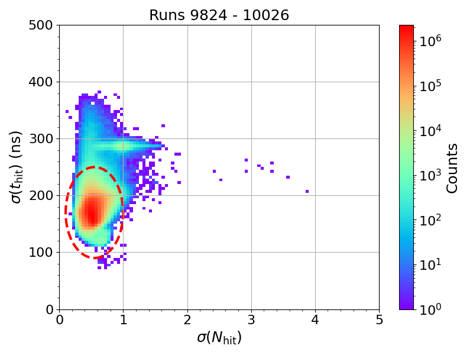
\includegraphics[width=0.5\linewidth]{3_background/fig_flasher_discriminate_quantities.png}
    \caption{2D distribution of $\sigma_{t_{\text{hit}}}$ v.s. $\sigma_{N_{\text{hit}}}$. Select CD triggers with $E_\text{rec}\in(0.7, 12]~\mathrm{MeV}$ after cosmic-ray muon veto from physics runs. The ellipse cut region is marked with the red dashed line.}
    \label{fig:flasherdistribution}
\end{figure}

Beyond the ellipse cut region, the CD triggers are considered "nonphysical", which are mainly contributed by the flashers. About 0.05 Hz events are cut off in normal runs. By assuming that all cut off events are physical triggers, we can estimate that the upper limit on the inefficiency is less than 0.1\% (shown in fig \ref{fig:flasherinefficiency}). Runs with a rate higher than this are classified as 'abnormal' due to their flasher-rich nature. Unlike normal runs, abnormal runs show a distinct peak caused by flashers. As shown in fig \ref{fig:flashercontamination}, the separation between physical events and flashers becomes clearer as the energy increases. There may be a inflection point between the peaks formed by physical events and flashers. The contamination from remaining flashers, estimated by extending the inflection point into the signal region, does not exceed 0.05\% in the worst case.

\begin{figure}[htbp]
    \centering
    \begin{subfigure}[b]{0.19\textwidth}
        \centering
        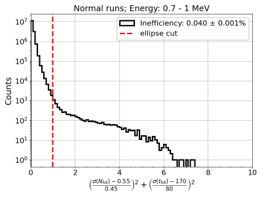
\includegraphics[width=\textwidth]{3_background/fig_flasher_inefficiency_0.7-1.png}
    \end{subfigure}
    \begin{subfigure}[b]{0.19\textwidth}
        \centering
        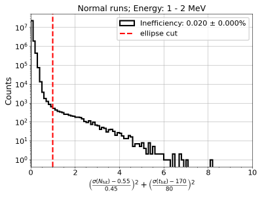
\includegraphics[width=\textwidth]{3_background/fig_flasher_inefficiency_1-2.png}
    \end{subfigure}
    \begin{subfigure}[b]{0.19\textwidth}
        \centering
        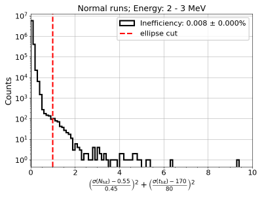
\includegraphics[width=\textwidth]{3_background/fig_flasher_inefficiency_2-3.png}
    \end{subfigure}
    \begin{subfigure}[b]{0.19\textwidth}
        \centering
        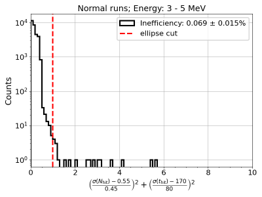
\includegraphics[width=\textwidth]{3_background/fig_flasher_inefficiency_3-5.png}
    \end{subfigure}
    \begin{subfigure}[b]{0.19\textwidth}
        \centering
        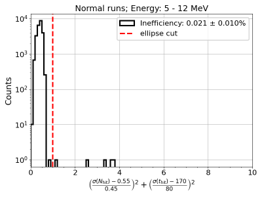
\includegraphics[width=\textwidth]{3_background/fig_flasher_inefficiency_5-12.png}
    \end{subfigure}
    \caption{CD physical triggers inefficiency of flasher cut in different energy ranges. $\epsilon$ distributions of normal runs are used. }
    \label{fig:flasherinefficiency}
\end{figure}

\begin{figure}[htbp]
    \centering
    \begin{subfigure}[b]{0.19\textwidth}
        \centering
        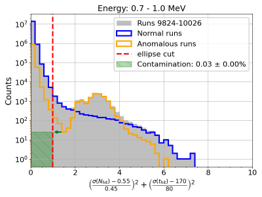
\includegraphics[width=\textwidth]{3_background/fig_flasher_contamination_0.7-1.png}
    \end{subfigure}
    \begin{subfigure}[b]{0.19\textwidth}
        \centering
        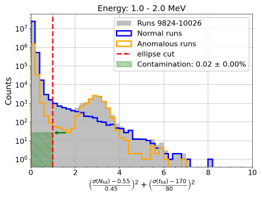
\includegraphics[width=\textwidth]{3_background/fig_flasher_contamination_1-2.png}
    \end{subfigure}
    \begin{subfigure}[b]{0.19\textwidth}
        \centering
        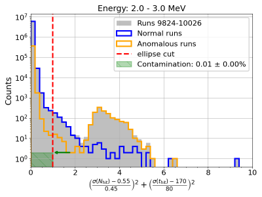
\includegraphics[width=\textwidth]{3_background/fig_flasher_contamination_2-3.png}
    \end{subfigure}
    \begin{subfigure}[b]{0.19\textwidth}
        \centering
        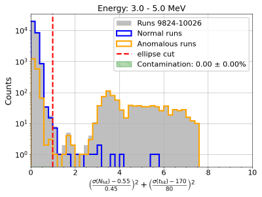
\includegraphics[width=\textwidth]{3_background/fig_flasher_contamination_3-5.png}
    \end{subfigure}
    \begin{subfigure}[b]{0.19\textwidth}
        \centering
        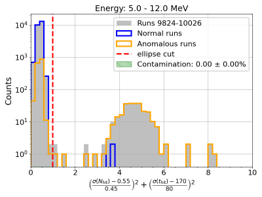
\includegraphics[width=\textwidth]{3_background/fig_flasher_contamination_5-12.png}
    \end{subfigure}
    \caption{Flasher contamination after cut in different energy ranges. Green regions are the extension of inflection point, which can be seen as the remained flashers.}
    \label{fig:flashercontamination}
\end{figure}

%\td{Uncertainty and inefficiency for IBD? Need selected IBD's distribution}

\subsection{Accidental background}
The accidental background was determined using an time-offwindow method. This technique employs selection criteria identical to the standard IBD analysis, except for the coincidence time window applied to the prompt and delayed signals. We pair delayed-like events with prompt-like candidates taken from time windows far away from the true coincidence region. For each delayed candidate that passes the muon and multiplicity vetoes, the algorithm shifts the delayed time backward by 2, 10, 12, 17, and 30 s, forming 500 off-time windows (100 windows for each main time offset). Within each shifted window, a virtual delayed signal is placed at the edge of the window, and we search for prompt-like events that satisfy the same energy, spatial, and time-difference cuts as real IBD pairs. Both the delayed and prompt candidates must also pass their own muon and multiplicity vetoes, ensuring that no muon or nearby activity occurs within the veto windows before or after each candidate. The scheme is shown in Fig.~\ref{fig:off_window}.

\begin{figure}
    \centering
    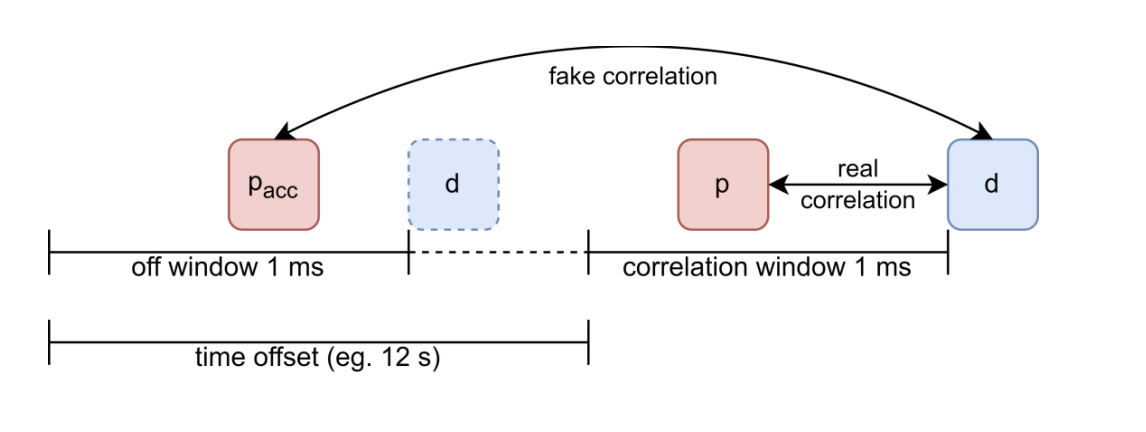
\includegraphics[width=0.8\linewidth]{2_selection/off_window_scheme.png}
    \caption{The scheme of the off-window method. }
    \label{fig:off_window}
\end{figure}

The time-offwindow method requires additional selections and corrections. Although it follows the same selection strategy as the standard IBD selection, the impact of muon-related backgrounds differs. In the standard IBD selection, the prompt signal is close to the delayed signal and thus well separated from muons. But in the time-offwindow method, the prompt signal can be close to muons. We apply an additional muon veto and multiplicity cut on the virtual delayed signal and correct the efficiency, to make sure the results from both selections consistent. This procedure was validated using simulation dataset as shown in Fig.~\ref{fig:off_window_correction}..

\begin{figure}
    \centering
    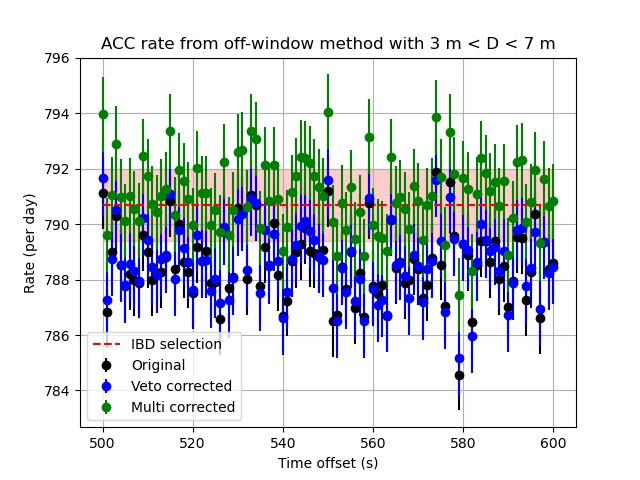
\includegraphics[width=0.7\linewidth]{3_background/rate_off_window_500s_fastn_fv176_eos.png}
    \caption{Validation of the correction on time-offwindow method with released distance cut. The difference is decreased from 0.26\% to 0.04\% after correction.}
    \label{fig:off_window_correction}
\end{figure}

The accidental background was found to be 0.049$\pm$0.003 counts per day for the fiducial volume $r<16.5$~m, |z|<15.5~m. The uncertainty of this measurement is dominated by the statistical uncertainty in the event rate measured within the off-time window. The results are shown in Fig.~\ref{fig:ACC_rate_shape} and Fig.~\ref{fig:ACC_vertex}.

\begin{figure}[!htbp]
    \centering
    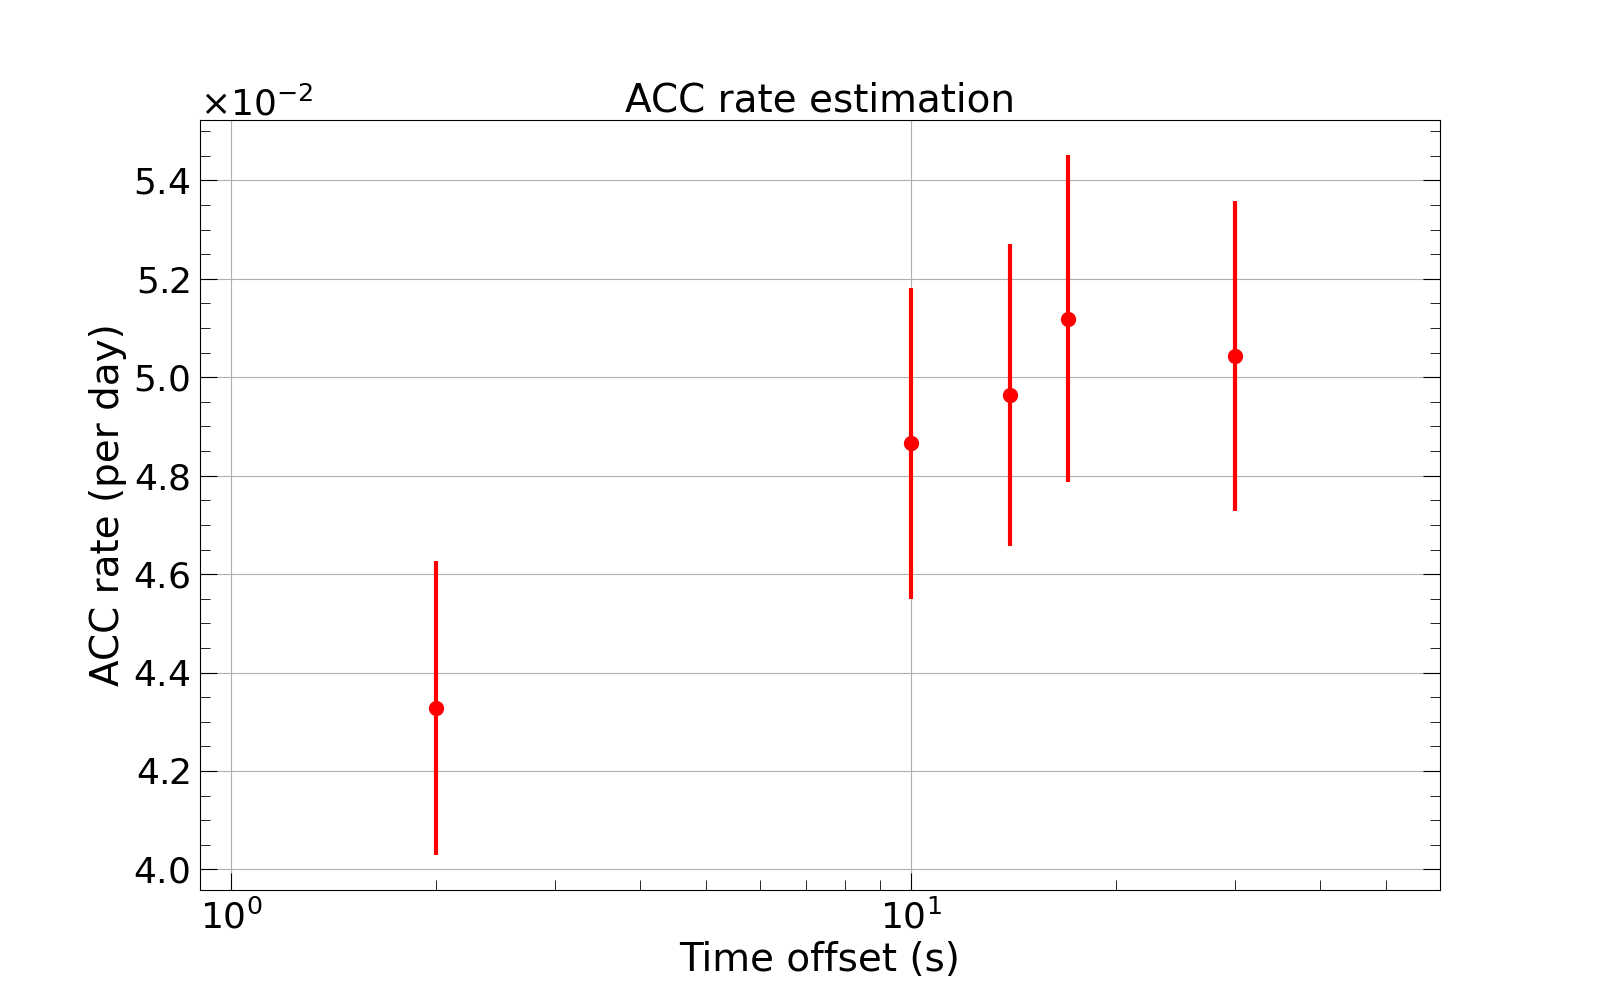
\includegraphics[width=0.49\textwidth]{3_background/h_good_d_15_rate_acc_main_eff.png}
    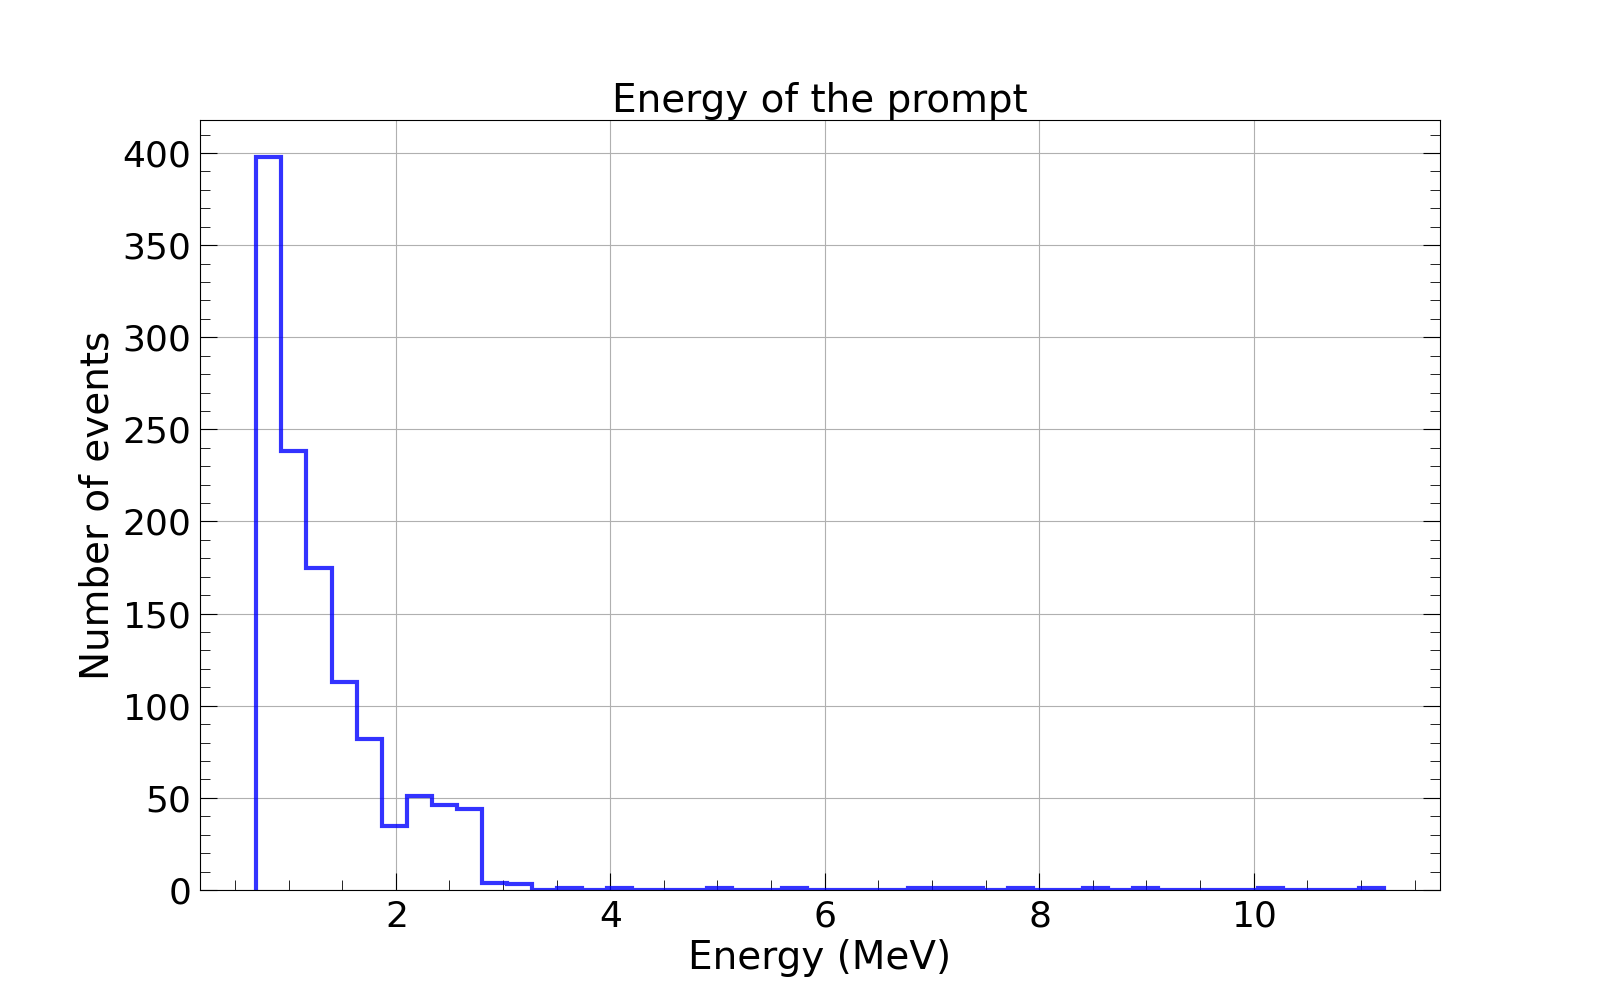
\includegraphics[width=0.49\textwidth]{3_background/h_good_d_15_e_p_0.png}
    \caption{Left: Estimated rate with extra veto and multiplicity cut efficiency correction. Right: Energy spectrum of the prompt signal of accidental coincidence background.}
    \label{fig:ACC_rate_shape}
\end{figure}

\begin{figure}[!htbp]
    \centering
    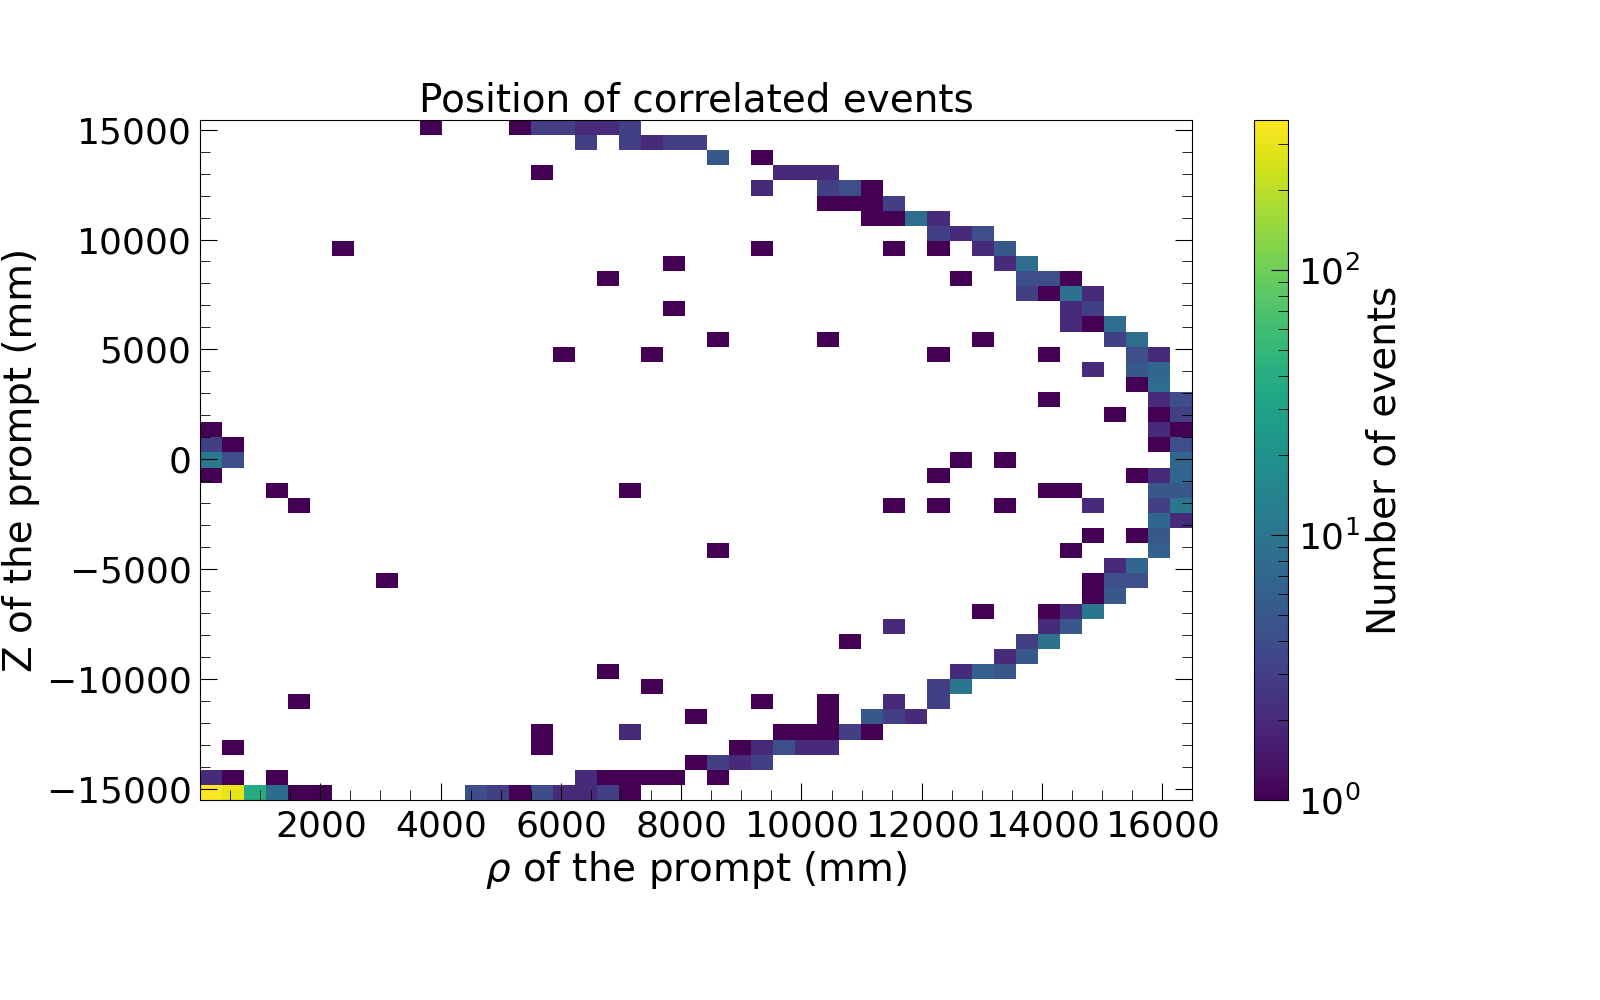
\includegraphics[width=0.49\textwidth]{3_background/h_good_d_15_rho_z_p_0.png}
    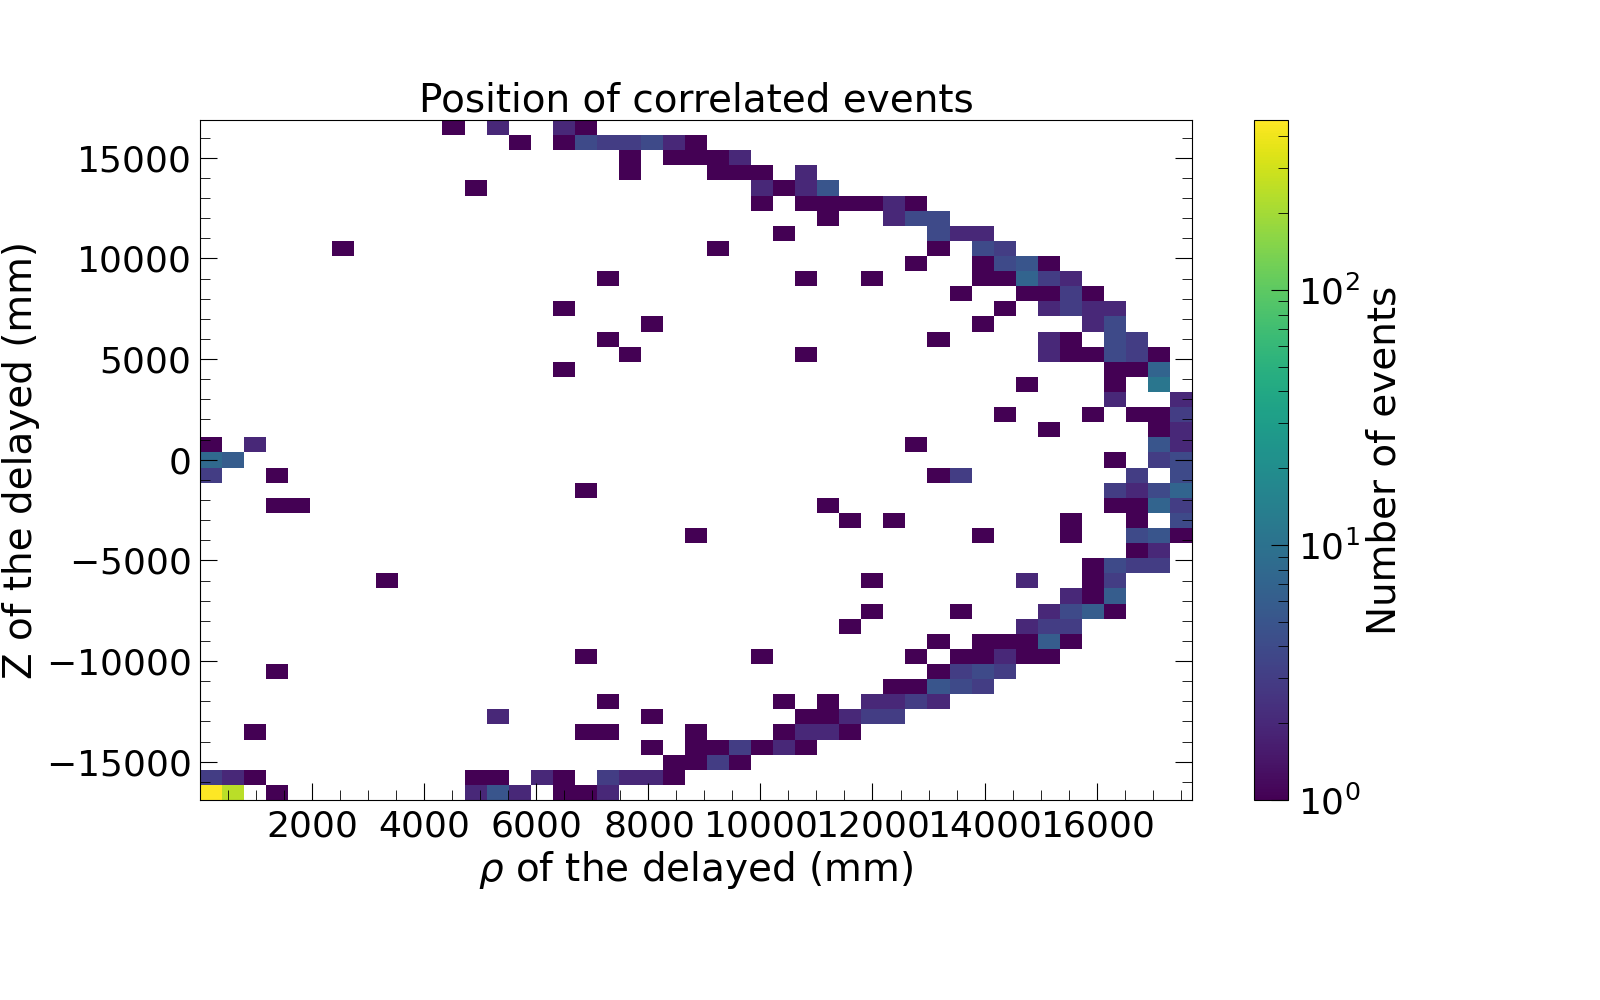
\includegraphics[width=0.49\textwidth]{3_background/h_good_d_15_rho_z_d_0.png}
    \caption{Vertex distribution of the prompt and delayed signals selected by off-window method.}
    \label{fig:ACC_vertex}
\end{figure}

\subsection{\Li}
Cosmogenic induced spallation isotopes on $^{12}$C in the LS can become a correlated background for IBD. Among them, $^9$Li and $^8$He are the dominant ones, each with a branching ratio of 51\% and 16\% $\beta$-neutron cascade decay. The $\beta$ decays have a Q value of 13.6 MeV for $^9$Li and 10.7 MeV for $^8$He. They have a relatively long half-life of 178.0 ms and 119.0 ms, respectively \cite{nndc}. The $^{9}$Li/$^{8}$He yield is derived from a time-since-last-muon fit, as it is produced by muon unlike the IBD. More details on the methods can be found in \cite{li9_doc_db}.

\subsubsection{Yield evaluation}
% \textcolor{red}{numbers are to update with ReprodB}

The dataset used in this results is based on the same one for IBD selection, i.e. ReProd25C with OMIREC reconstruction. An IBD sample is prepared with the same selection criteria as A1, but no spallation neutron veto or any shower muon veto to retain $^{9}$Li/$^{8}$He in the sample. The muon is defined as a CD trigger (Q>3e4 PE) with a correlated WP trigger (Q>1e3 PE) within $\pm$5$\mu$s. The time since last muon distribution is fitted by the following function:

\begin{equation}
    N(t) = \sum_{iso}N_{iso}\lambda_{iso}e^{-\lambda_{iso}t} + N_\mathrm{(IBD+Acc+iso2)}R_\mu e^{-R_\mu t}
\end{equation}

where $iso$ runs over $^9$Li, $^8$He, $\lambda_{iso}=R_\mu+1/\tau_{iso}$, and $R_\mu$ is the muon rate. $N_\mathrm{IBD+Acc+iso2}$ represents IBD events, Accidental events and $^{9}$Li/$^{8}$He uncorrelated to the muon. The fraction between the number of $^8$He and $^9$Li events is fixed to be 0.0143. The time since the last muon fit does not work when the muon rate is high. In Figure~\ref{fig:time_fit_li9}, example fits are shown for the time since the last muon of different visible energies. The fitted muon rates are consistent with the rates calculated by counting. $^{9}$Li/$^{8}$He events are produced by muons with high-energy deposits during showers. Clear $^{9}$Li/$^{8}$He are fitted for muon energy larger than 1e7 pe ($\sim$5 GeV). For muon energy smaller than 1e7 PE, the fit gives a much smaller number of $^{9}$Li/$^{8}$He, the error is very large due to a much worse $^{9}$Li/$^{8}$He to IBD ratio. We also tried to float the lifetime of $^{9}$Li/$^{8}$He, and the fitted lifetime is consistent with $^{9}$Li/$^{8}$He lifetime within uncertainties.

To properly take into account the correlations between the four time-since-last-muon distributions in different muon energy slices, a joint fit of the four energy slices is performed. The fitted error is also cross checked with another MC and  bootstrap methods. And they are found consistent. 

\begin{figure}
    \centering
    \includegraphics[width=0.8\linewidth]{3_background/time_fit_li9_example.png}
    \caption{Time since last muon fit for different muon visible energy (PE) regions: [1e6, 7e6], [7e6, 1e7], [1e7, 1.2e7], [1.2e7, 2e9] (from left to right, top to down). }
    \label{fig:time_fit_li9}
\end{figure}

To increase the $^{9}$Li/$^{8}$He event purity in the IBD sample, we require events with $E_p>6$ MeV. The results is summarized in Figure~\ref{fig:fitted_rate_comp}. The fraction of events with with $E_p>6$ MeV over $E_p>0.7$ MeV 0.40$\pm$0.06, compared to the predictions of 0.40/0.36 from DYB/common input. Note that the results for $E_{p}$ $>$ 0.7 MeV in Figure~\ref{fig:fitted_rate_comp} are derived from direct fitting.

For $^{9}$Li/$^{8}$He events generated by $Q_\mu$<5e6 PE, we use the correction factor from MC truth \cite{li9_doc_db}. After taking into account the selection efficiency ($\sim$0.6988) as well \cite{li9_doc_db}, the $^{9}$Li/$^{8}$He yield ($\beta$-$n$ branch) is evaluated to be 73.6$\pm$2.7 cpd. This yield is derived from the total fitted SPN-tagged events plus the residual events following SPN veto.

\begin{figure}
    \centering
    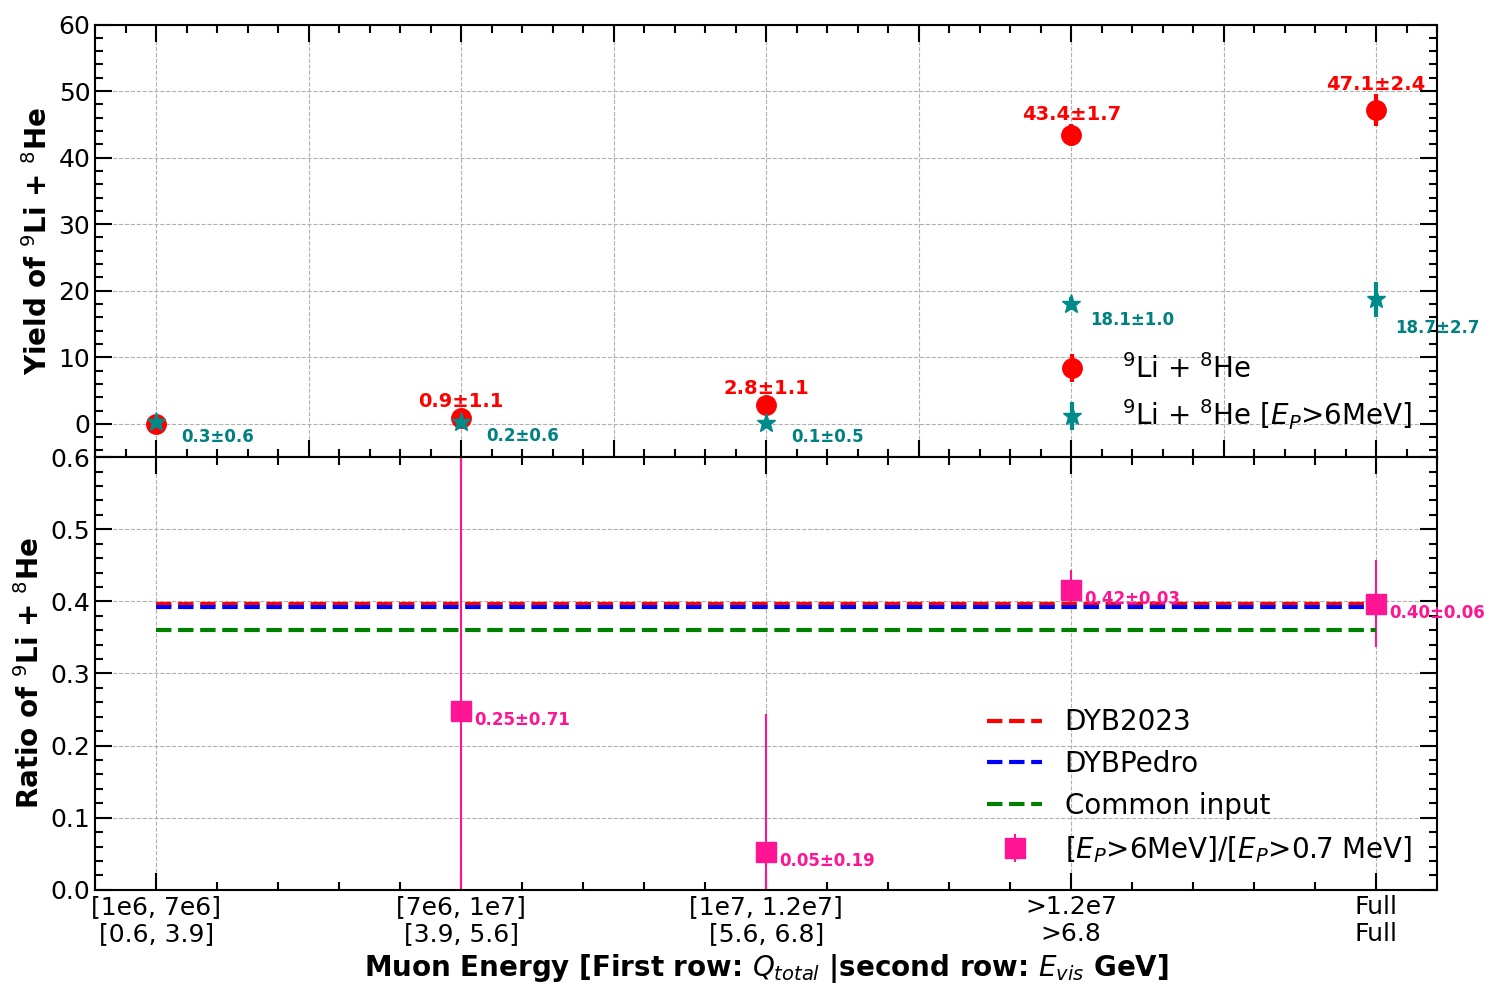
\includegraphics[width=0.7\linewidth]{3_background/fitted_rate_comp_w_Ep_gt_6MeVnew.png}
    \caption{Fitted $^{9}$Li/$^{8}$He rate comparison with a prompt energy cut of $>$6 MeV.}
    \label{fig:fitted_rate_comp}
\end{figure}

% \begin{table}[!htbp]
%     \caption{\Li rate summary.}
%     \label{tab:li9}
%     \centering
%     \begin{tabular}{c|cccc}
%         \hline
%         Muon energy [PE] & $<$5e6 & [5e6, 1e7] & [1e7, 2e7] & $>$2e7 \\
%         \hline
%         Livetime [day] & \multicolumn{4}{c}{33.1} \\
%         \hline
%         Counts      & 51$\pm$34  & 0$\pm$80  & 333$\pm$82 & 1087$\pm$41  \\
%         Rate [cpd]  &   &   &   & \\
%         \hline
%         Counts (Ep>6 MeV)  & 23$\pm$18  & 0$\pm$11  & 118$\pm$49 & 473$\pm$25 \\
%         Rate [cpd]   &   &   &   & \\
%         \hline 
%     \end{tabular}
% \end{table}


\subsubsection{Veto strategy and residual background}
\Li~is often produced accompany with neutrons. Therefore, we use a spallation neutron (spn) veto to remove \Li~events in this analysis. The spn is tagged with the following criteria: [20, 2000] $\mu$s after muon, and 3000 PE$<Q_\mathrm{spn}<$ 30000 PE. %(This are slightly different from the A1 IBD selection, will converge in the next update).% 
The neutron peak energy cut is relaxed to account for the events impacted by afterpulses after large muon events. For each identified spn, a sphere veto of 4m radius around the spn vertex within 1.2 s is implemented. 

\begin{figure}
    \centering
    \includegraphics[width=0.8\linewidth]{3_background/time_fit_w_spn_veto.png}
    \caption{fit results after spn veto for different muon visible energy (PE) regions: [1e6, 7e6], [7e6, 1e7], [1e7, 1.2e7], [1.2e7, 2e9] (from left to right, top to down). }
    \label{fig:spn_veto}
\end{figure}

The remaining \Li~is evaluated by time since the last muon fit. The result is summarized in Figure~\ref{fig:spn_veto_rate_summary}. More than 97\% \Li~ events are rejected for the $Q_\mu$>1.2e7 PE region. The rejection for lower energy slice is worse. An overall 90\% of \Li~events are rejected in total. The residual \Li~event rate after veto is $4.3\pm1.4$ (after efficiency correction: $6.2\pm2.1$) cpd. The dominant residual contribution are from two medium energy regions from 5e6 to 1.2e7 PE. 
%This could be due to the CTU threshold increase after muon events. For lower energy muon events, the afterpulse impact is smaller and the spn can not pass the trigger threshold. One possible improvement in the future is to lower the after-muon CTU threshold for low energy muons. 

\begin{figure}
    \centering
    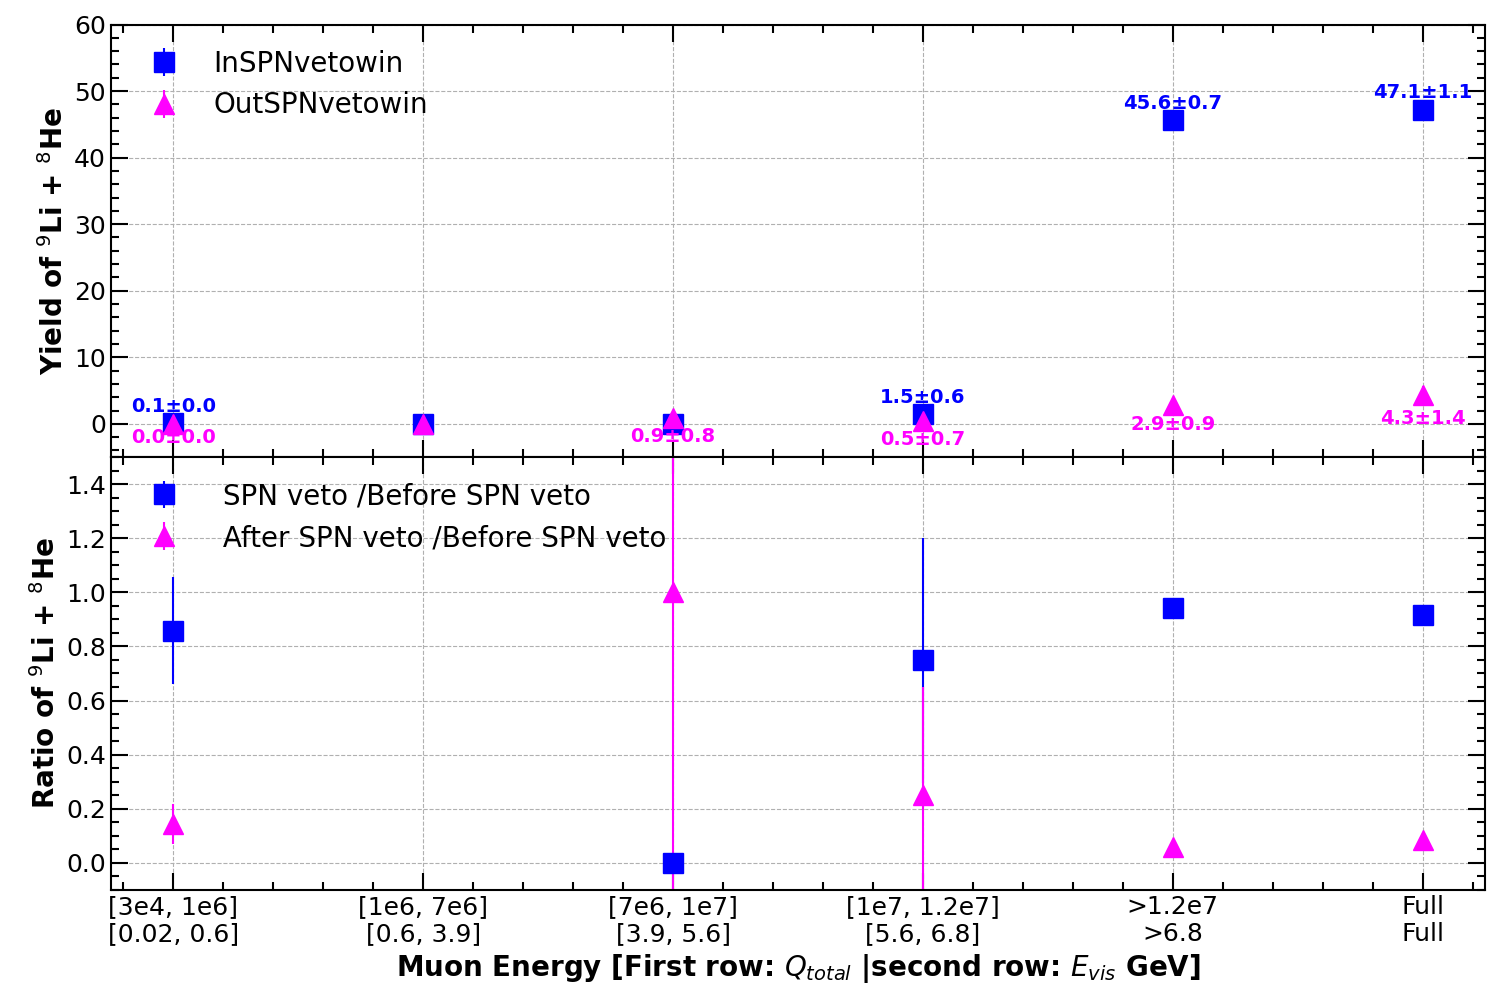
\includegraphics[width=0.8\linewidth]{3_background/spn_veto_rate_summarynew.png}
    \caption{\Li~event rate summary with spn veto.}
    \label{fig:spn_veto_rate_summary}
\end{figure}


% \begin{table}[!htbp]
%     \caption{\Li rate summary after spallation neutron veto.}
%     \label{tab:li9_after_veto}
%     \centering
%     \begin{tabular}{c|cccc}
%         \hline
%         Muon energy [PE] & $<$5e6 & [5e6, 1e7] & [1e7, 2e7] & $>$2e7 \\
%         \hline
%         Livetime [day] & \multicolumn{4}{c}{33.1} \\
%         \hline
%         Counts      & 17$\pm$23  & 71$\pm$42  & 80$\pm$56  & 35$\pm$17  \\
%         Rate [cpd]  &   &   &   &   \\
%         Rate [cpd]  & \multicolumn{4}{c}{6.1$\pm$\td{error from combined fit}} \\
%         \hline
%         Counts (Ep>6 MeV)   & 15$\pm$8  & 23$\pm$14  & 41$\pm$24  & 25$\pm$9 \\
%         Rate [cpd]          &   &   &   & \\
%         \hline
%         Residual [cpd]  &   &   &   &   \\
%         \hline 
%     \end{tabular}
% \end{table}
\subsubsection{MC comparison}
To compare the yields of $^9$Li and $^8$He with those from the GEANT4-v11 simulation, we first establish a calibration between the measured muon visible energy and simulated muon energy loss. Figure~\ref{fig:mueloss} demonstrates that the simulated muon energy loss in the liquid scintillator agrees with the muon visible energy in real data within the energy range of 0.5 GeV to tens of GeV. This agreement is achieved after scaling the simulation by a factor of 1.7$\times$10$^6$ photoelectrons per GeV to obtain the total charge. Using this established relationship and applying the same veto  strategy in the simulation, we then determined the yields for $^9$Li and $^8$He.
\begin{figure}
    \centering
    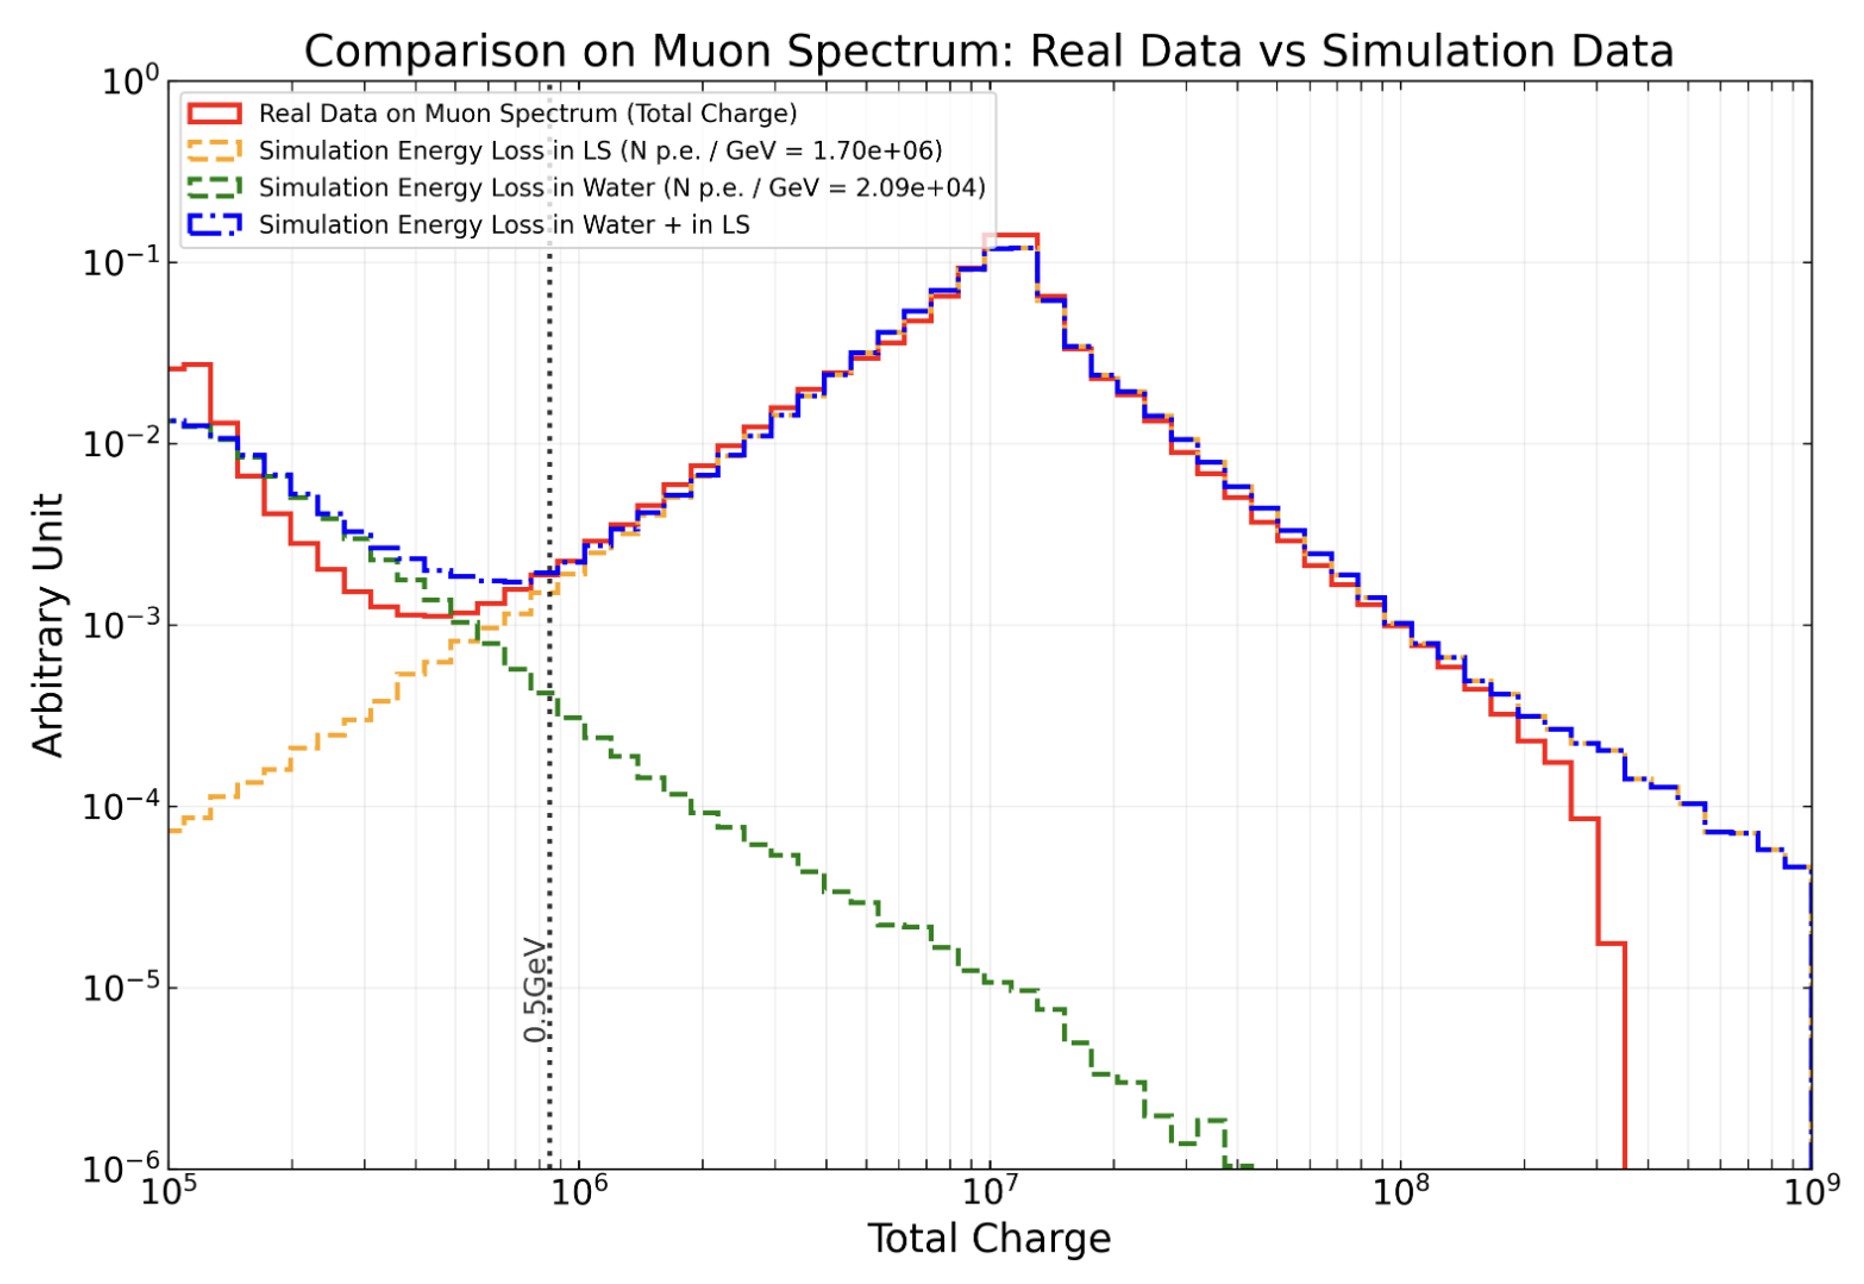
\includegraphics[width=0.8\linewidth]{3_background/muonEloss.png}
    \caption{The simulated muon energy loss in the liquid scintillator matches the muon visible energy in real data well.}
    \label{fig:mueloss}
\end{figure}

Figure~\ref{fig:li9mc} compares the yields of both residual and total $^9$Li and $^8$He from the MC and real data after applying corrections for detector efficiency and muon rate. The residual yields in the IBD sample show good agreement between the simulation and data.
\begin{figure}
    \centering
    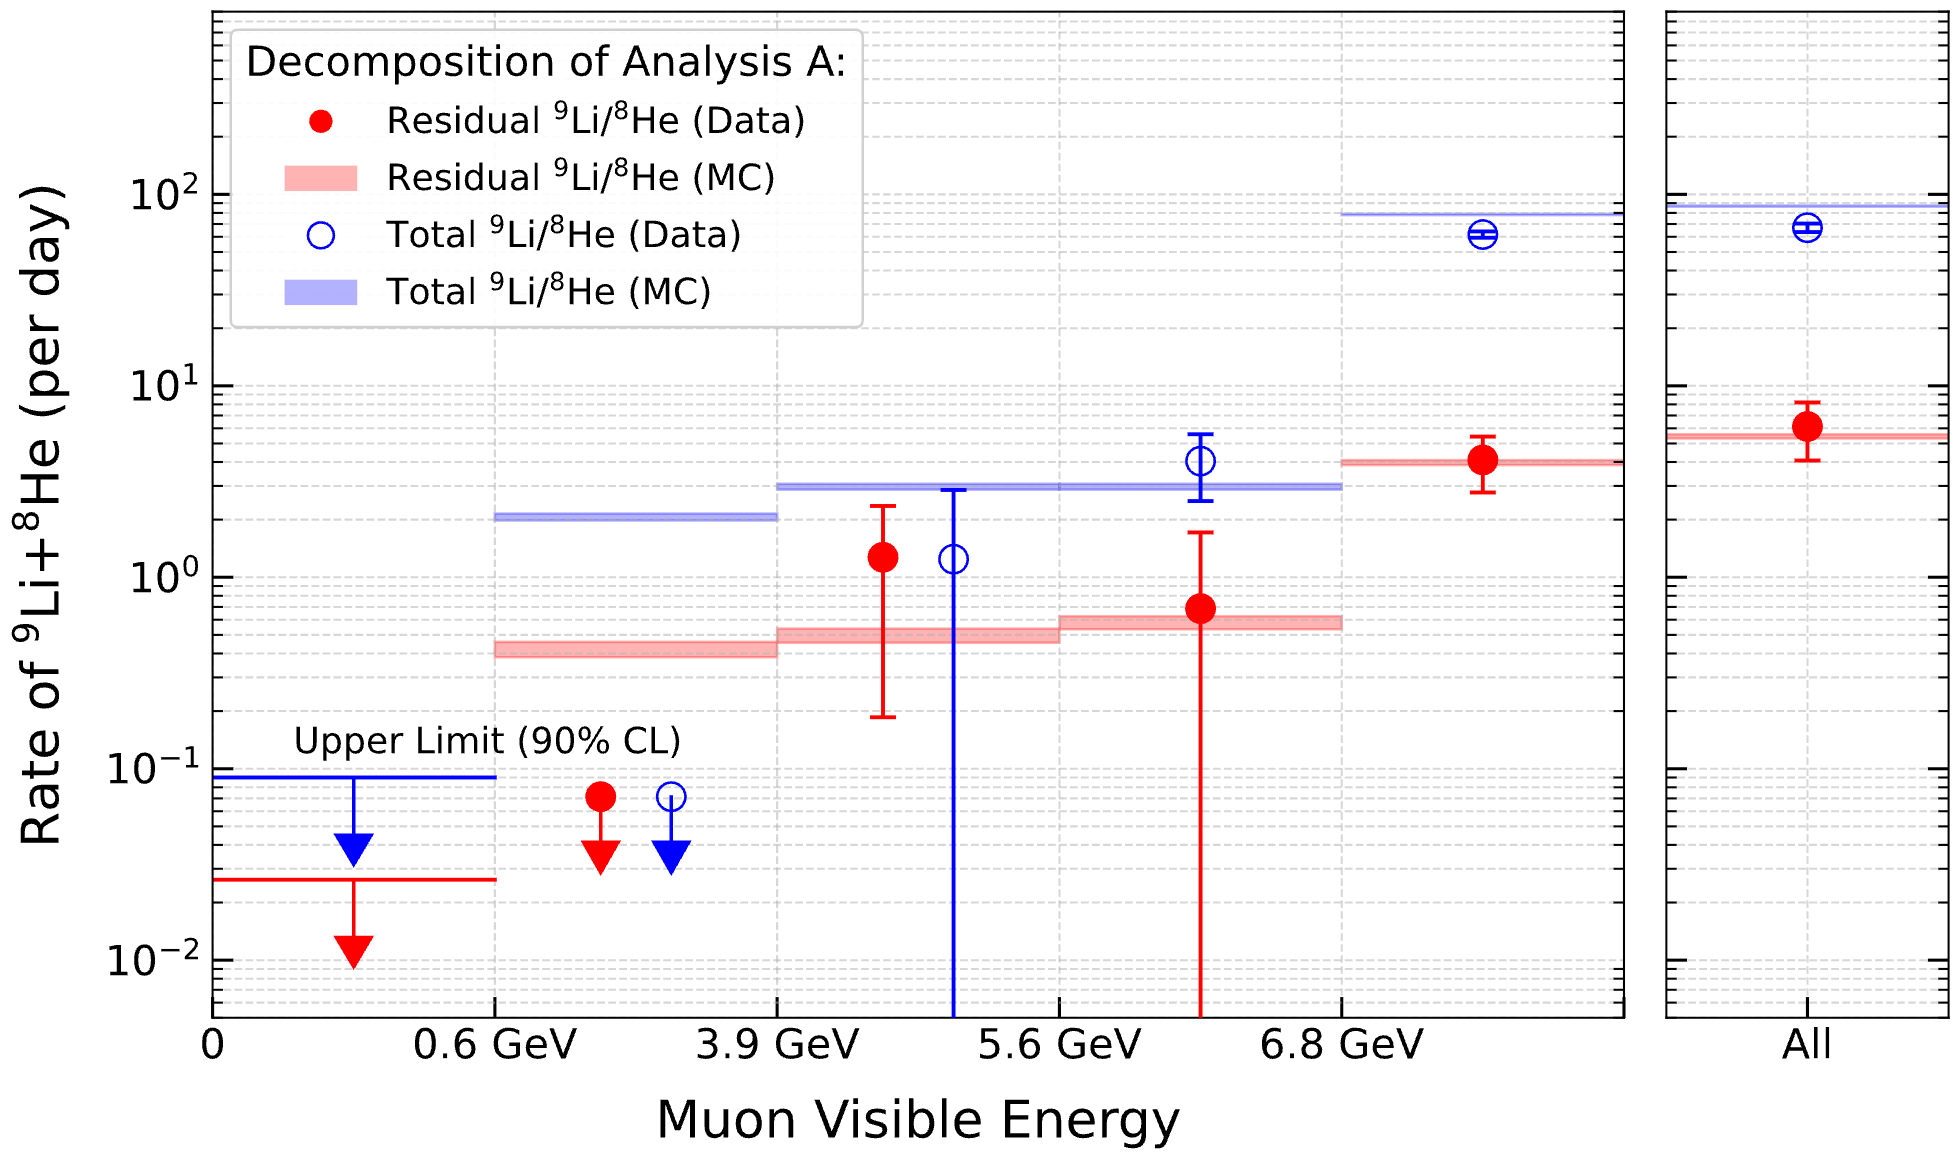
\includegraphics[width=0.8\linewidth]{3_background/li9mc.png}
    \caption{ The comparison of the simulation and real data for the yields of $^9$Li and $^8$He.}
    \label{fig:li9mc}
\end{figure}

\subsubsection{Energy Spectrum}

$^{9}$Li/$^{8}$He energy spectrum can be measured from data in-situ, using SPN-correlated sample. The results are shown in Figure~\ref{fig:li9_spec}, which the corresponding muon energy is $>$ 1.2$\times$10$^7$ pe. Figure~\ref{fig:li9_spec} shows the measured and different predicted energy spectrum. In the left plot, differences between the data and models are presented. A new theoretical modeling of $^9$Li spectrum is proposed in \cite{li9_spec}, and shown in Figure~\ref{fig:li9_spec}. It takes special account into the distribution of the excited states of the intemediate $^9$Be, $^5$He and $^8$Be. These differences are generally small, with deviations of < 20\% for most data points. Additionally, statistical fluctuations dominate the observed discrepancies.
% The measured data spectrum have a reasonable agreement with the predictions above 6 MeV. A clear discrepancies around 3 MeV are  shown for different predictions. 

The right plot presents a comparison of the predicted energy spectra for $^{9}$Li/$^{8}$He from different models. The relative differences between these spectra are generally < 20\%, except energies below 2 MeV, where the discrepancy originates from the DYB2023 model. Finally, through the synthesis of data-model comparisons and inter-model comparisons, the overall uncertainty is determined to be 20\%.
 % The nominal $^9$Li spectrum for the fit will be based on CZ's modeling, constrained by the spn tagged data. The shape error will take into account the difference from data and the several models. The detailed implementation is in progress.
\begin{figure}
    \centering
    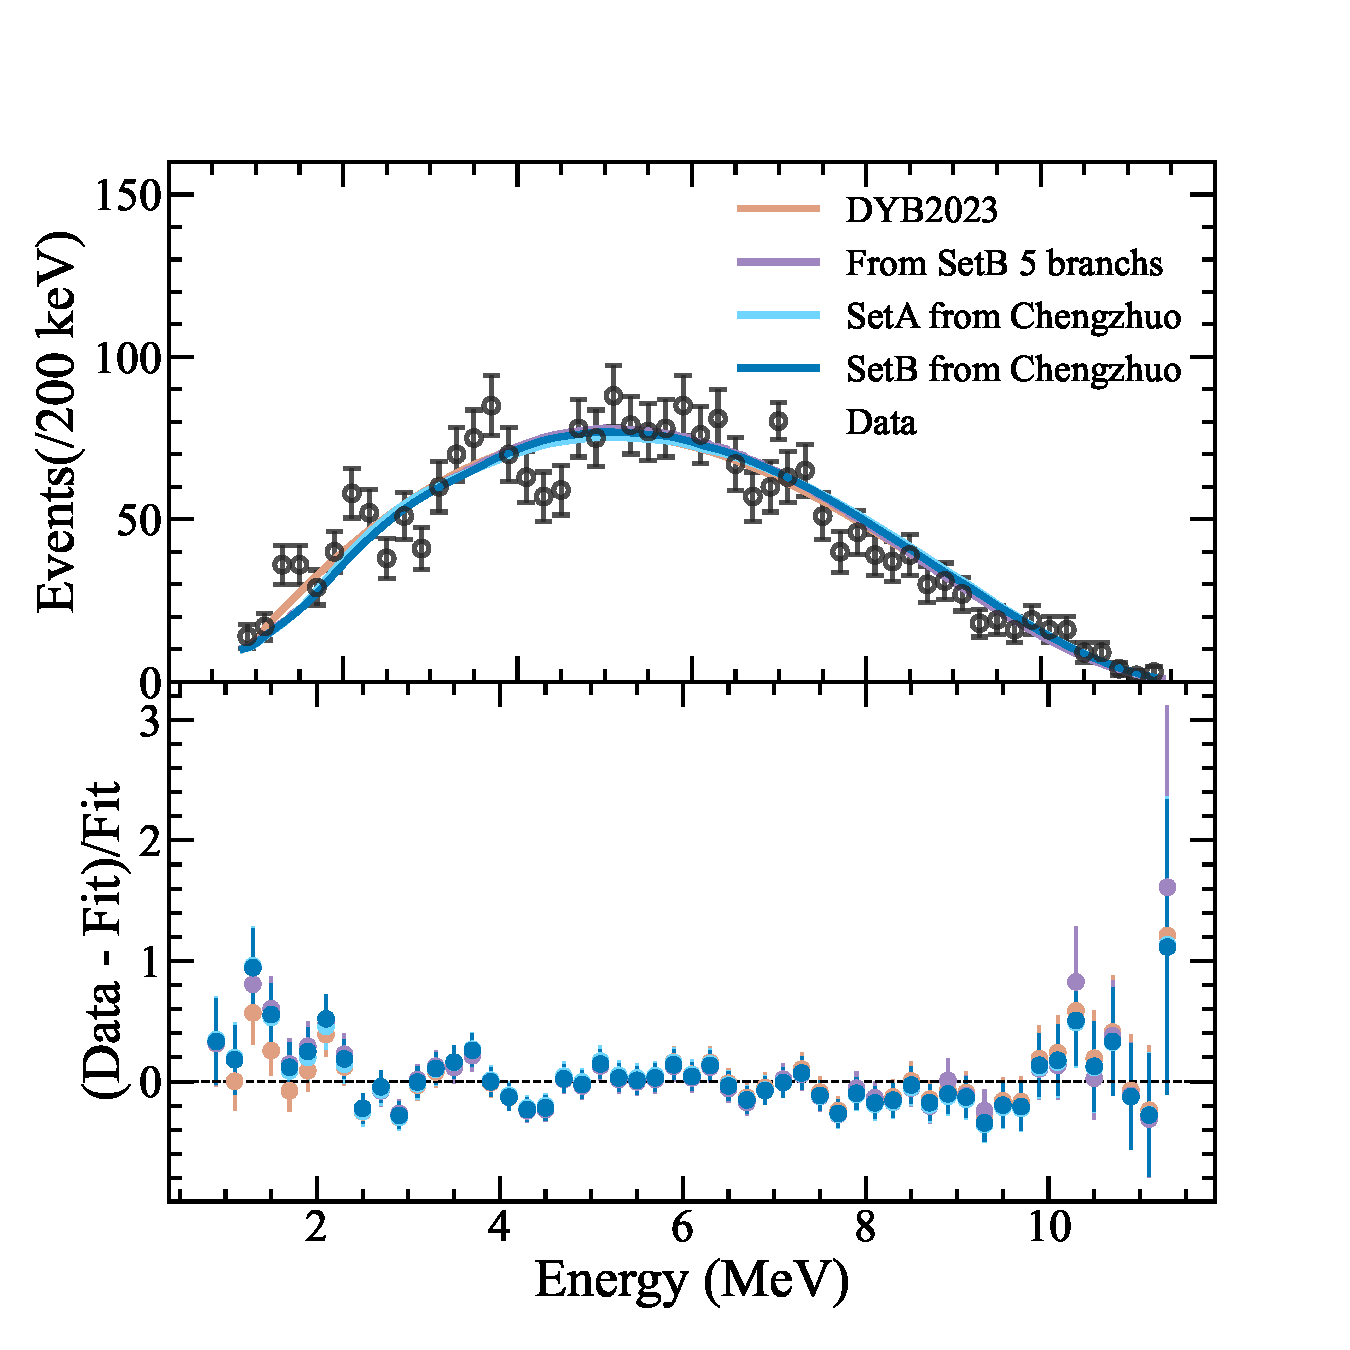
\includegraphics[width=0.45\linewidth]{3_background/Li9energyspectra_comdatamodels.pdf}
    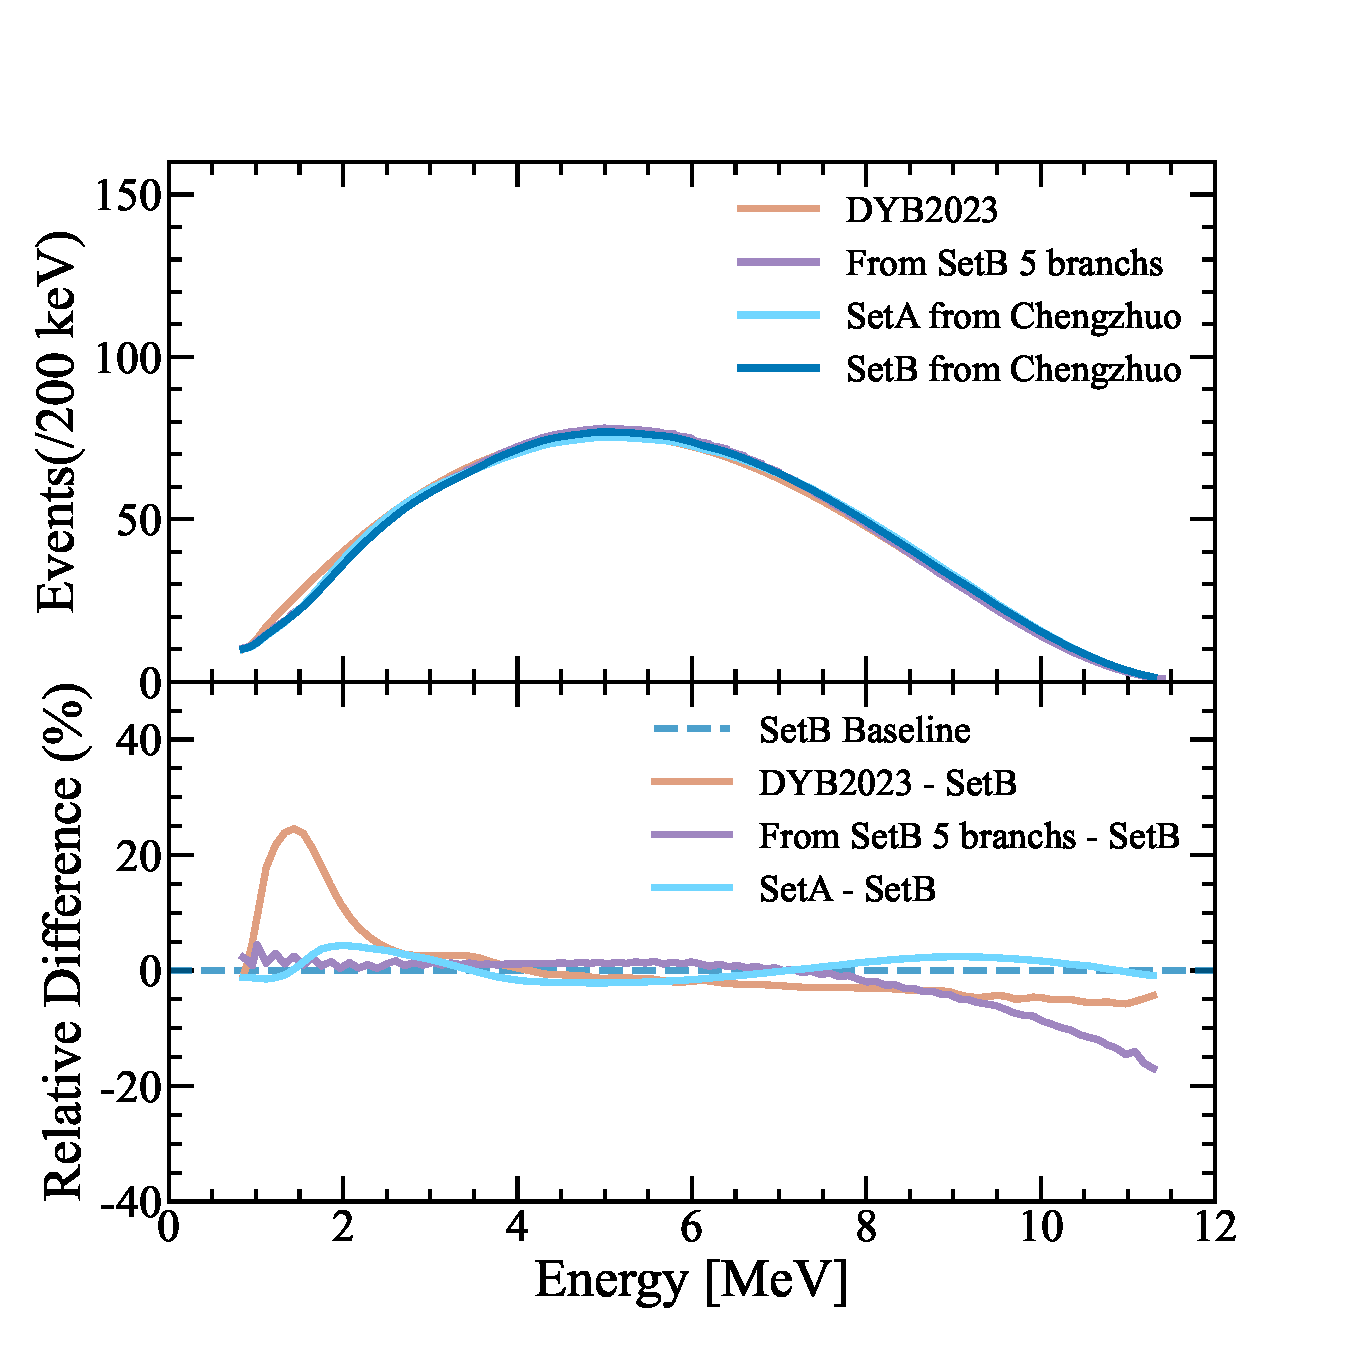
\includegraphics[width=0.45\linewidth]{3_background/Li9energymodelcompare.pdf}
    \caption{$^{9}$Li/$^{8}$He spectrum measured from data and predictions. The measured energy spectrum is tagged by high energy muon with energy larger than 1.2e7 pe, which gives a high purity sample. The left plot shows the results of data and three models. The right plot are predictions from the DYB2023 and sets from Chengzhuo. Model differences are presented in the lower panel of the right plot.}
    \label{fig:li9_spec}
\end{figure}

% \begin{figure}
%     \centering
%     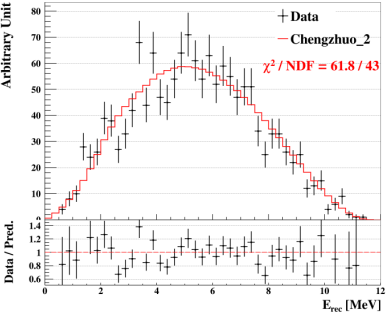
\includegraphics[width=0.6\linewidth]{3_background/li9_CZ.png}
%     \caption{Comparison of the $^9$Li spectrum tagged with spn and the new prediction from Chengzhuo.}
%     \label{fig:li9_CZ}
% \end{figure}

\subsection{Fast neutrons/double neutrons}

  Energetic neutrons generated by cosmic-ray muons represent a background in the JUNO experiment, mainly through two distinct mechanisms: single fast neutrons and double neutron captures. Fast neutrons can imitate an Inverse Beta Decay (IBD) event via elastic scattering off a proton (producing a prompt signal) followed by capture on hydrogen (yielding a delayed signal). Similarly, double neutrons constitute a correlated background in which a muon produces two separate neutrons that are subsequently captured, generating a prompt-like signal from the first neutron’s capture and a delayed signal from the second.
\subsubsection{Rate}
This study employs a comprehensive methodology that integrates Monte Carlo simulations with real-data analysis. The fast neutron selection cut used: prompt energy[0.7,12]MeV, delay energy[2.1,2.5]MeV, prompt signal time [0,2us] from last muon, prompt and delay signal time difference [1,1500]us. The Fidual volume (FV) cut, R<16.5 and |Z|<15.5m. One Monte Carlo dataset(1168-day MC data), containing only rock muons was used, yielding a fast-neutron rate of approximately 0.02/day and a double-neutron rate of 0.05/day, with a total rate below 0.1/day. The spectrum is shown in Figure~\ref{fig:fastn}. Both fast and double-neutron backgrounds are found to be strongly concentrated near the detector’s periphery, rendering them highly sensitive to the fiducial volume cut. Given the low statistical counts for both fast neutrons and double neutrons, a conservative uncertainty of 100\% has been assigned to the rate evaluation.A fast-neutron rate of approximately 0.02$\pm$0.02/day and a double-neutron rate of 0.05$\pm$0.05/day, 
 
\begin{figure}[h]
    \centering
    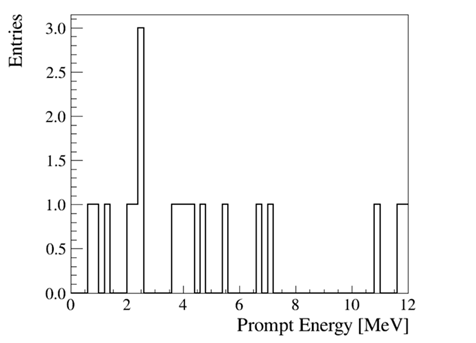
\includegraphics[width=8cm]{3_background/fastn-prompt.png}
    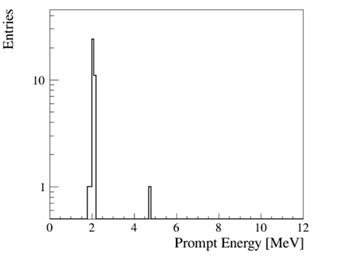
\includegraphics[width=8cm]{3_background/doublen_prompt.png}
    \caption{The prompt energy spectrum for fast neutron(Left figure) and double neutron(Right figure) from MC}
    \label{fig:fastn}
\end{figure}


% \begin{figure}[h]
 %   \centering
 %   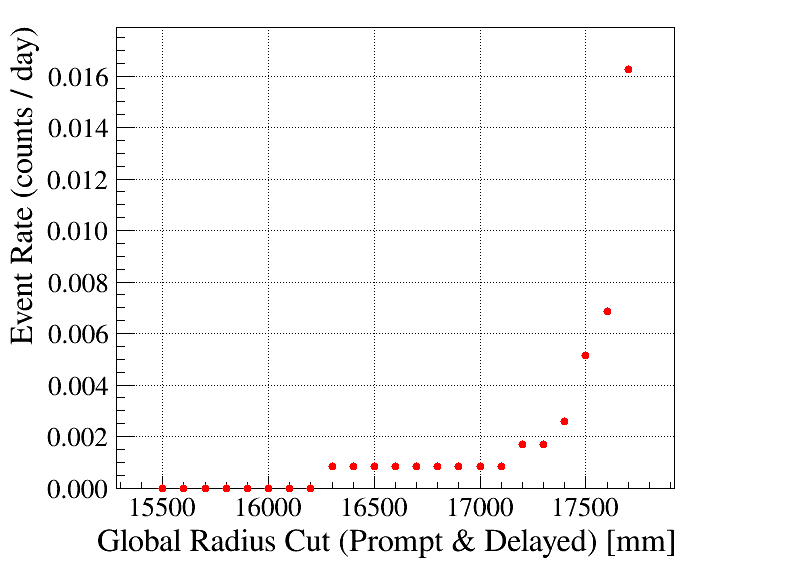
\includegraphics[width=8cm]{3_background/fastn-R.png}
 %   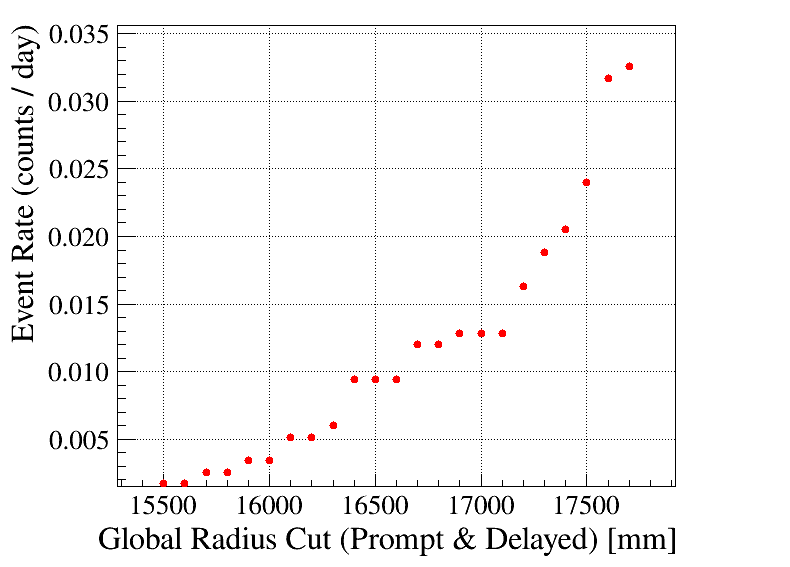
\includegraphics[width=8cm]{3_background/doublen-R.png}
 %   \caption{fast neutron(Left figure) and double neutron(Right figure) background vs detector radius}
 %   \label{fig:fastnR}
%\end{figure}
 

To validate and enrich these findings, real data are employed. A dedicated sample of corner-clipping muons from the Water Pool (with WP PE < 1000 and nHit > 250) is selected to estimate background levels. In an initial dataset spanning ~61 days, 1 fast neutron candidate was observed, while 4 double-neutron candidates were identified. For double neutrons, the expected coincidence events from IBD and Li9 decays within the selection window amount to approximately 4 event. Thus, no significant double-neutron background is observed during this data-taking period. 

\subsubsection{Spectrum}      
   For the energy spectrum study, since both the MC and data statistics are not enough. we intend only to select the high-energy neutrons energy deposited(proton recoil) spectrum to get more statistics, and only select the energy deposited with [0,2us] and FV<16.9 m without other cuts. Since the low statistics, we use a flat fit function to describe the fast-n spectrum.
  For the double neutron prompt signal spectrum from a neutron capture, we'll use the IBD delay signal neutron capture spectrum. The prompt energy spectrum for fast neutron and double neutron will be used, as shown in Fig.~\ref{fig:fastN-spectrum}. 
  
  The energy spectrum uncertainty of fast neutrons was evaluated by comparing the results from a constant linear fit and a first-order polynomial fit, with the discrepancy between these two functions yielding a conservative uncertainty estimate of 60\%. For the double neutron spectrum, the peak shifter error of the calibration source located inside the detector was less than 1\%. By shifting the entire spectrum upward and downward by 1\% and comparing it with the original spectrum, an approximate uncertainty of 50\% was derived.
   \begin{figure}[h]
    \centering
    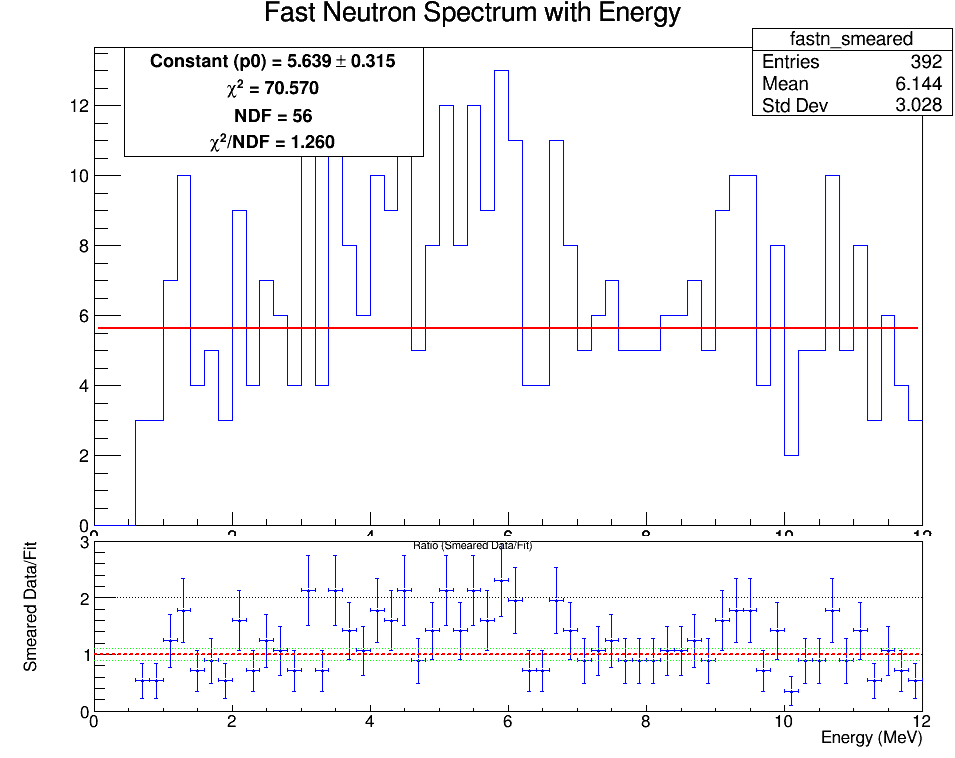
\includegraphics[width=7cm]{3_background/fastn_PromptSpectrum.png}
    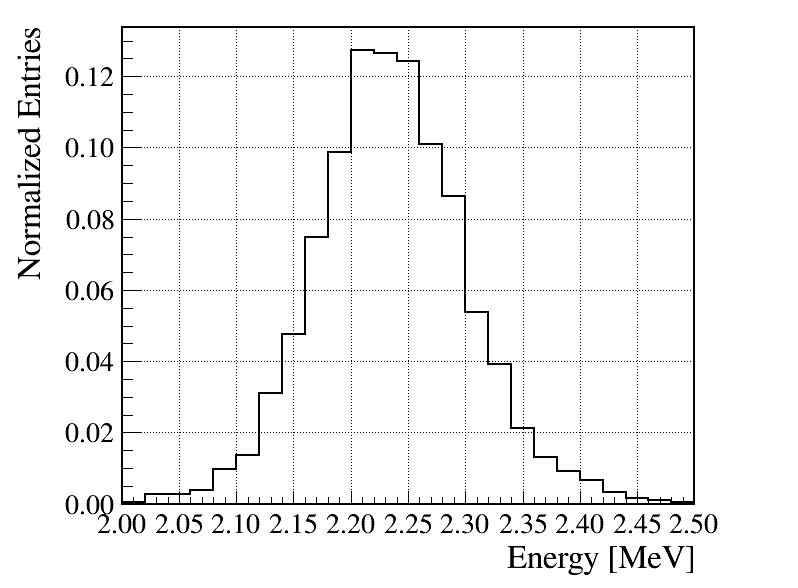
\includegraphics[width=8cm]{3_background/doublen_promptSpectrum.png}
    \caption{fast neutron prompt energy spectrum(Left figure) and double neutron prompt energy spectrum(Right figure) }
    \label{fig:fastN-spectrum}
\end{figure}
 

\subsection{Double $^{12}$B and other potential cosmogenic isotopes}
Cosmogenic isotopes produced by muons traversing the detector, constitute a significant background in IBD analyses. These isotopes are predominantly generated in proximity to muon tracks, often accompanied by neutron production due to muon-induced spallation. The temporal and spatial correlation among isotopes originating from the same muon event enables their effective identification as correlated pairs. In this section, we systematically investigate all potential cosmogenic isotopes that contribute to correlated pair formations (see DocDB: 14926), followed by a discussion of additional $\beta$--$n$ background (see DocDB: 14951) beyond the previously studied $\mathrm{^{9}Li}$ and $\mathrm{^{8}He}$.

\subsubsection{Observation of correlated events in extened delayed-energy window}
\begin{figure}[htbp]
		\centering
		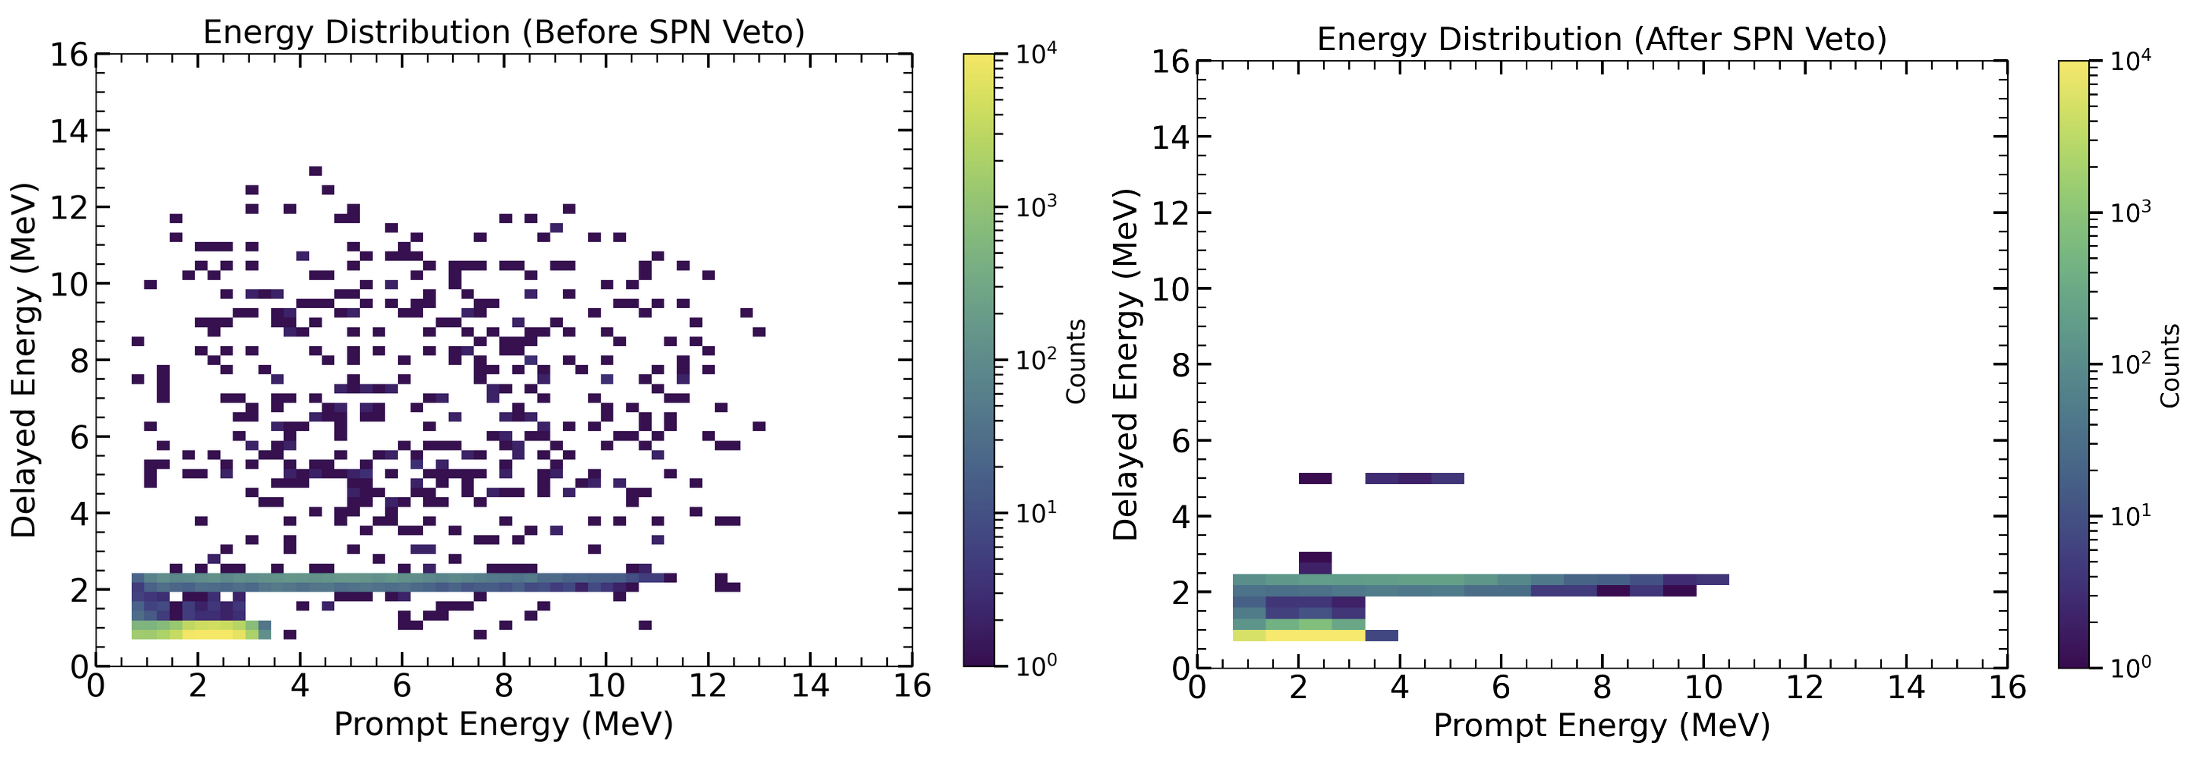
\includegraphics[width= 0.80\columnwidth]{3_background/B12extendeddelayed.png}
		\caption{During the IBD selection process, expanding the energy window for delayed signals reveals additional correlated events with delayed energies exceeding 3 MeV. We observe a reduction in correlated events exhibiting delayed energies exceeding 3 MeV after SPN veto compared to the previous analysis, attributable to the inclusion of muon information from bad files.}
        \label{fig:extendde}
\end{figure}
When the delay energy window in the IBD selection is extended, additional correlated events with delayed energies exceeding 3~MeV become observable, as illustrated in Figure~\ref{fig:extendde}. These events can mimic genuine IBD signals within the neutron capture energy region, necessitating a combined analysis of simulation and experimental data to accurately extrapolate the background rate.
\subsubsection{Paired particle types with $\mathrm{^{12}B}$}
Based on the observed production rates, energy spectra, and lifetimes, the majority of these correlated events before SPN veto are attributed to $\mathrm{^{12}B}$. In this study, we concentrate primarily on $\mathrm{^{12}B}$, with other isotopes addressed in subsequent analyses. To ensure consistency between simulation and experimental data, identical selection criteria are applied in the simulation, including a 5 ms muon veto window, pairing cuts, and multiplicity cuts. 


Figure~\ref{fig:b12time} shows the comparison of real data and MC results for the time difference relative to muons. Red points represent real data obtained from the delayed signal delay time to the closest muon, and are in good agreement with the blue MC points corresponding to pairs involving $\mathrm{^{12}B}$. Purple points denote double $\mathrm{^{12}B}$ events, while yellow points denote pairs involving $\mathrm{^{12}B}$ with other particle components. The lifetime extraction from fits to the comprehensive $\mathrm{^{12}B}$ dataset (green points) yields 29{ms}, aligning with the expected value. However, its production rate in simulation is notably lower than that in real data, suggesting the need for improved calibration of muon induced isotope yields.

\begin{figure}[htbp]
		\centering
		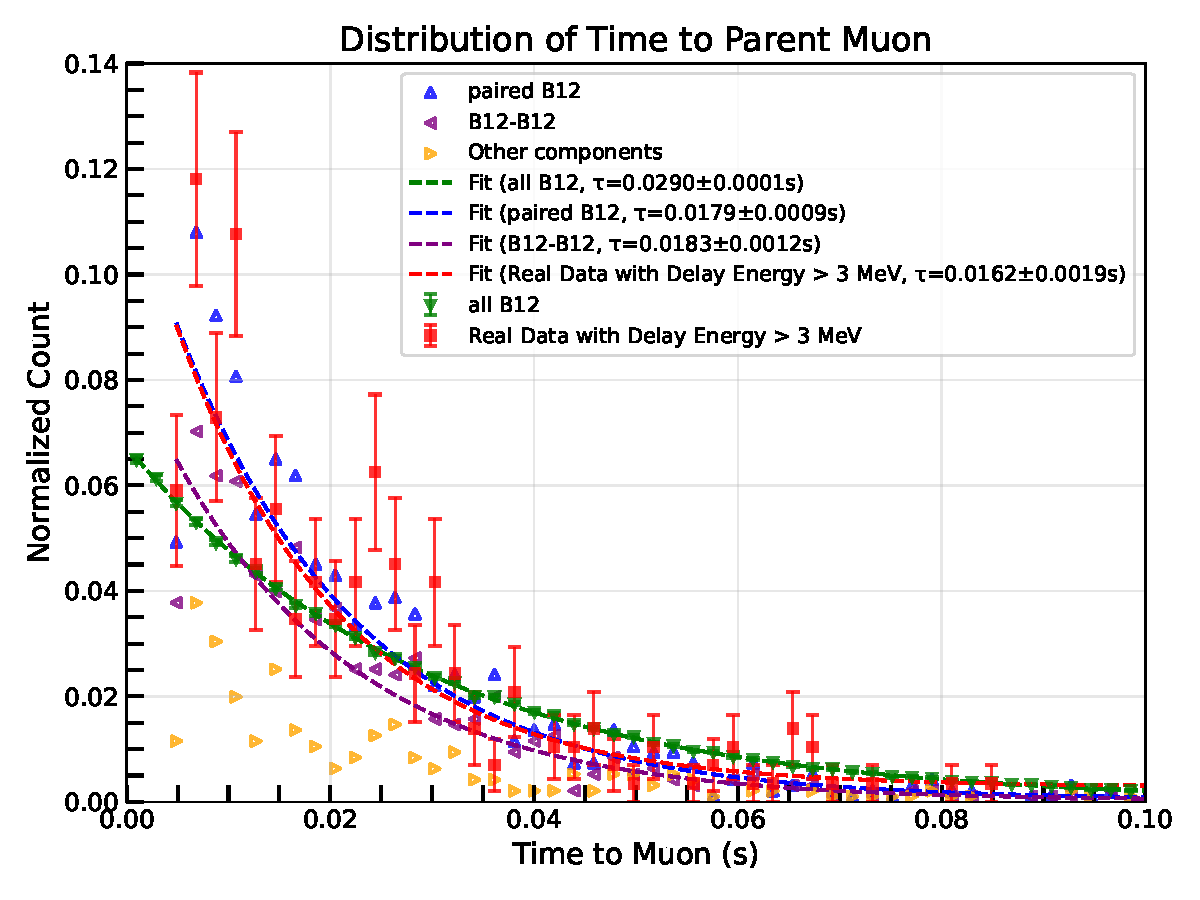
\includegraphics[width= 0.60\columnwidth]{3_background/B12t2mu.pdf}
		\caption{Comparison of time differences relative to the parent muons between the data and MC. Red points correspond to data, obtained from the delayed signal with respect to the nearest muon in time. Blue points correspond to pairs with B12 in the simulation. Purple points denote double-B12 events (B12–B12 pairs) in the MC, while yellow points represent pairs containing other particle components; both purple and yellow points are normalized to the count of blue-marked paired events. Green points show all B12 data in the MC, normalized to its total count.}
        \label{fig:b12time}
\end{figure}


\begin{table}[htbp]
\centering
\begin{tabular}{|l|c|c|}
\hline
\textbf{Paired particle with $\mathrm{^{12}B}$} & \textbf{Paired rate before spn veto(cpd)} & \textbf{Proportion} \\
\hline
$\mathrm{^{12}B}$   & 5.10 & 69.9\% \\
\hline
$\mathrm{^{12}N}$   & 1.03 & 14.2\% \\
\hline
$\mathrm{^{9}C}$    & 0.39 & 5.4\% \\
\hline
$\mathrm{^{8}Li}$   & 0.26 & 3.6\% \\
\hline
$\mathrm{^{6}He}$   & 0.21 & 2.8\% \\
\hline
$\mathrm{^{8}B}$    & 0.21 & 2.9\% \\
\hline
$\mathrm{^{10}C}$   & 0.03 & 0.4\% \\
\hline
$\mathrm{^{11}C}$   & 0.02 & 0.2\% \\
\hline
$\mathrm{^{9}Li}$   & 0.02 & 0.3\% \\
\hline
$\mathrm{^{8}He}$   & 0.02 & 0.2\% \\
\hline
neutron             & 0.01 & 0.1\% \\
\hline
$\mathrm{^{11}Be}$  & 0.00 & 0.0\% \\
\hline
$\mathrm{^{16}N}$   & 0.00 & 0.0\% \\
\hline
\textbf{Total}      & \textbf{7.27} & \textbf{100\%} \\
\hline
\end{tabular}
\caption{Paired particle types with $\mathrm{^{12}B}$ and their contributions before SPN veto over a 150-day Geant4-10 simulation sample.}
\label{tab:b12}
\end{table}


Table~\ref{tab:b12} summarizes the particle types paired with $\mathrm{^{12}B}$ in a 150-day simulation sample. After scaling to match the muon rate observed in real data, the total pairing rate is approximately 7.3 cpd, with the majority of paired signals consisting of double $\mathrm{^{12}B}$ combinations.
\subsubsection{Correlated events including all potential cosmogenic isotopes}
\begin{table}[htbp]
\centering
\begin{tabular}{|l|c|c|}
\hline
\textbf{Paired Particle} & \textbf{Rate before spn veto (cpd)} & \textbf{Rate after spn veto (cpd)} \\
\hline
$\mathrm{^{12}B}$ & 9.99 (7.27) & 0.01 (0.04) \\
\hline
$\mathrm{^{12}N}$ & 1.31 (1.17) & 0.004 (0) \\
\hline
$\mathrm{^{8}Li}$ & 0.82 (0.66) & 0.08 (0.05) \\
\hline
$\mathrm{^{9}C}$ & 0.17 (0.51) & 0 (0) \\
\hline
$\mathrm{^{6}He}$ & 0.92 (0.43) & 0.08 (0.02) \\
\hline
$\mathrm{^{8}B}$ & 0.12 (0.37) & 0.02 (0.02) \\
\hline
$\mathrm{^{10}C}$ & 0.18 (0.15) & 0.06 (0.06) \\
\hline
$\mathrm{^{11}C}$ & 0.11 (0.03) & 0.08 (0) \\
\hline
$\mathrm{^{9}Li}$ & 0.21 (0.03) & 0 (0) \\
\hline
$\mathrm{^{8}He}$ & 0.04 (0.01) & 0 (0) \\
\hline
Be11 & 0 (0.01) & 0 (0.01) \\
\hline
N16 & 0 (0) & 0 (0) \\
\hline
\textbf{Total} & \textbf{10.92 (8.02)} & \textbf{0.23 (0.15)} \\
\hline
\end{tabular}
\caption{Correlated events rate including all potential cosmogenic isotopes with and without SPN veto over a 277.5-day Geant4-11 simulation sample (150-day Geant4-10 simulation sample in bracket).}
\label{tab:paired_table2}
\end{table}




We extend Table~\ref{tab:paired_table2} to include all potential isotopes, not only B12 in two simulation samples. Before the SPN veto, the total paired rate is 10.92 (8.02) cpd (with 9.99 (7.27) cpd attributed to B12 and Li-9/He-8 neutron pairings not included). After applying the SPN veto, the total is 0.23 (0.15) cpd.
\begin{figure}[htbp]
		\centering
		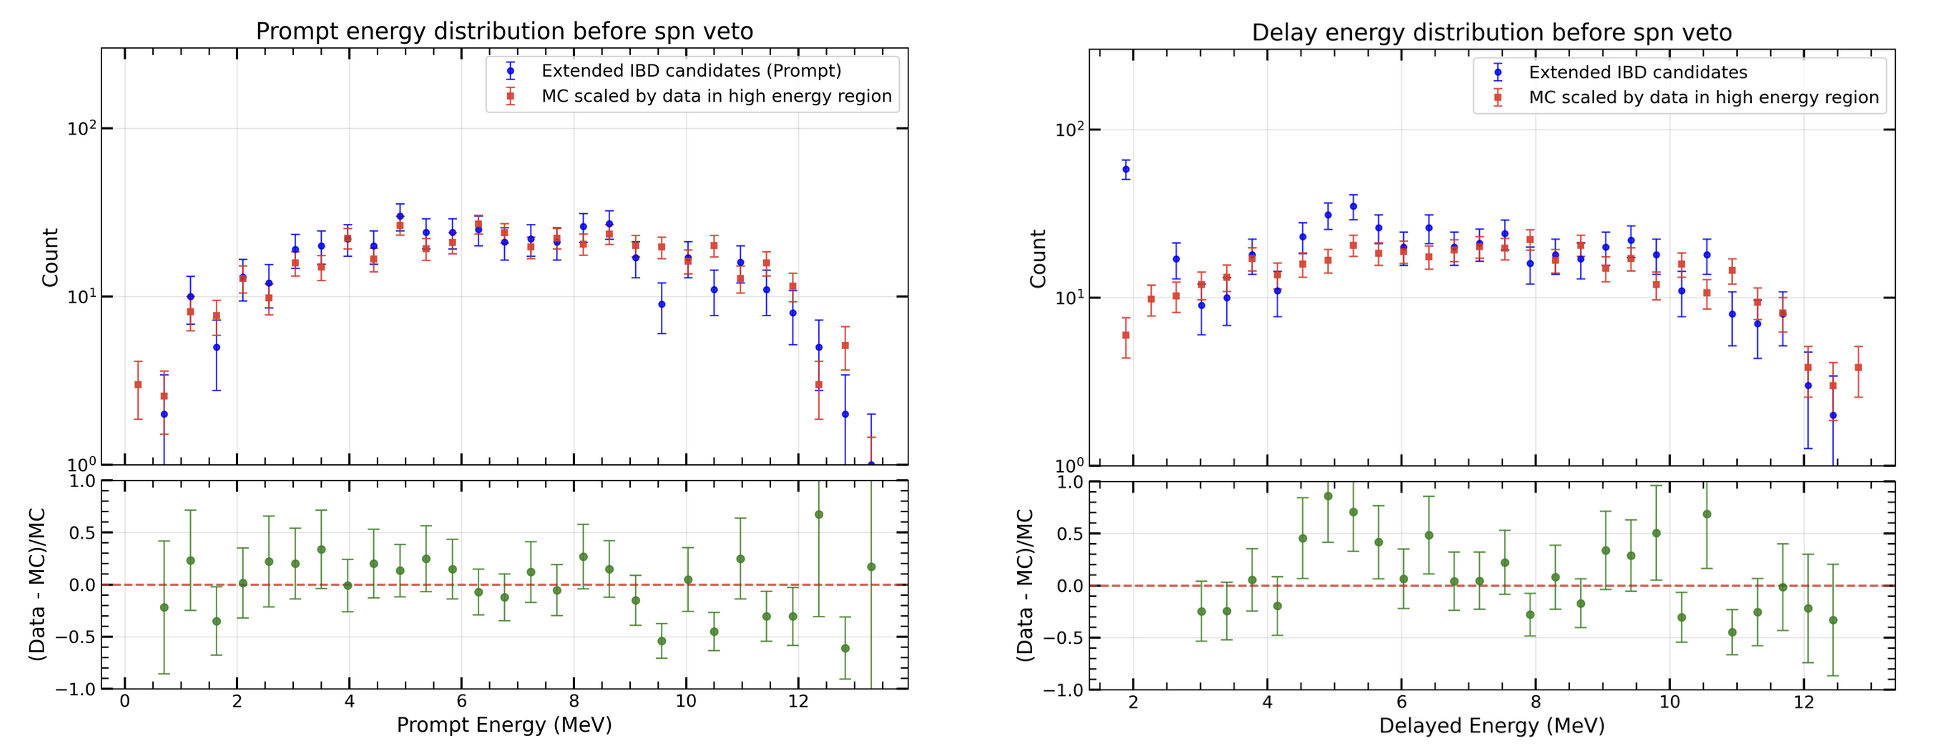
\includegraphics[width= 0.90\columnwidth]{3_background/B12spec.png}
		\caption{Extended delay energy spectrum and prompt energy spectrum for IBD candidates selection in real data (blue) and the scaled MC delay energy spectrum for correlated events from all potential cosmogenic isotopes (red).}
        \label{fig:b12delay}
\end{figure}




Two 59.1-day data samples were analyzed, one incorporating the spn veto and the other excluding it. 
Figure~\ref{fig:b12delay} shows the extended delay energy spectrum for IBD candidates selection (blue); the red curve shows the scaled MC delay energy spectrum for correlated events from all potential cosmogenic isotopes.
To extrapolate the IBD background in the 2.1–2.6 MeV delay energy interval, we employ the rate above 6 MeV threshold to suppress neutron capture events on carbon. 


\begin{table}[htbp]
\centering

\newcommand{\tabletitlewidth}{4.5cm}

\begin{tabular}{|l|c|c|}
\hline
\makebox[\tabletitlewidth][l]{\textbf{Before SPN veto ($\mathrm{E_d}$)}} & \textbf{$>6$ MeV} & \textbf{2.1--2.6 MeV} \\
\hline
G4-10 rate (cpd) & 4.65 $\pm$ 0.19 (stat.) & 0.28 $\pm$ 0.05 (stat.) \\
\hline
G4-11 rate (cpd) & 5.08 $\pm$ 0.14 (stat.) & 0.36 $\pm$ 0.05 (stat.) \\
\hline
Data rate (cpd) & 6.55 $\pm$ 0.40 (stat.) & \textbf{0.46 $\pm$ 0.07 (sys.) $\pm$ 0.11 (stat.)} \\
\hline
\end{tabular}

\vspace{0.3cm} 

\begin{tabular}{|l|c|c|}
\hline
\makebox[\tabletitlewidth][l]{\textbf{After SPN veto ($\mathrm{E_d}$)}} & \textbf{$>6$ MeV} & \textbf{2.1--2.6 MeV} \\
\hline
G4-10 rate (cpd) & 0.04 $\pm$ 0.02 (stat.) & 0.01 $\pm$ 0.01 (stat.) \\
\hline
G4-11 rate (cpd) & 0.04 $\pm$ 0.01 (stat.) & 0.01 $\pm$ 0.01 (stat.) \\
\hline
Data rate (cpd) & $<0.055$ (90\% CL)& \textbf{<0.014  (90\% CL)} \\
\hline
\end{tabular}

\caption{Rates before and after the SPN veto for two energy windows, with the 2.1–2.6 MeV IBD background extrapolated via the Geant4-10 and Geant4-11 simulation derived ratio.}
\label{tab:rates_ED_before}
\end{table}



Before the SPN veto, the rate for delay energy above 6 MeV is 6.55 cpd, slightly higher than the MC prediction as shown in Table~\ref{tab:rates_ED_before}. This difference can be explained by the data showing a $\mathrm{^{12}B}$ production rate higher than the expected rate from MC. Using the simulation derived IBD background ratio yields an extrapolated IBD background rate in data of 0.46 cpd, with a statistical uncertainty of 0.11 cpd, and a systematic uncertainty of 0.07 is estimated by comparing results from different simulation samples. 
After applying the SPN veto, no candidate events are observed. This allows us to establish a 90\% CL upper limit of 0.055 cpd on the signal rate for events with delayed energy > 6 MeV. The 90\% CL upper limit on the corresponding extrapolated IBD background is 0.014 cpd. As this limit is negligible, it was not included in the subsequent analysis.

\subsubsection{Cosmic ray induced ${\beta}$-n isotopes}
Beyond $\mathrm{^9Li}$ and $\mathrm{^8He}$, several $\mathrm{\beta}$-n isotopes produced by cosmic ray spallation can contribute to IBD like backgrounds in JUNO, including $\mathrm{^{11}Li}$, $\mathrm{^{12}Be}$, $\mathrm{^{14}B}$, $\mathrm{^{16}C}$, $\mathrm{^{17}N}$, and $\mathrm{^{18}N}$. For the long lived species such as $\mathrm{^{16}C}$, $\mathrm{^{17}N}$, and $\mathrm{^{18}N}$, their delayed neutron-emitting decays make vetoing by spallation neutrons or  muon track particularly challenging. Consequently, a quantitative assessment of this irreducible background relies on simulation. Using combined FLUKA and Geant4 simulations, we estimate the total $\mathrm{\beta}$-n background from isotopes excluding $\mathrm{^{17}N}$ to be approximately 0.02~cpd with a systematic uncertainty of about 40\%. The $\mathrm{^{17}N}$ $\mathrm{\beta}$-n background rate remains uncertain, as the two simulations differ by roughly an order of magnitude and require further cross-checking. Notably, $\mathrm{^{17}N}$ constitutes the dominant $\mathrm{\beta}$-n background despite the uncertainty, details can be found in DocDB: 14951.


\subsection{$^{13}$C($\alpha$, n)$^{16}$O}
%Done by Rongping.

$\alpha$ from natural radioactivity may interact with a nucleus and emit a neutron. The reaction, formed by X($\alpha$;n)Y, introduces background to the LS based neutrino experiments. In the LS detector, $\alpha$ comes from $^{238}$U, $^{232}$Th, and $^{210}$Po decay chains. The nucleus $^{13}$C is a natural component of Carbon which is rich in the LS. The $^{13}$C($\alpha$;n)$^{16}$O reaction
forms the correlation as following: the prompt signal is neutron elastic scattering on proton or inelastic scattering on $^{12}$C, and the delayed signal is neutron capture on Hydrogen. If $^{16}$O is in the excited state, de-excitation of $^{16}$O emits  or conversion electron which also contributes to the prompt signal. The signature is the same as $\overline{\nu}_e$, so such events can't be distinguished from $\overline{\nu}_e$ samples. The background rate and spectrum should be subtracted carefully from the neutrino candidates.

\subsubsection{Neutron yield and spectrum}
A newly developed generator code for calculating the alpha-n yield has been developed by Rongping (IHEP), details can be found in Doc14912. The difference of this method to SaG4n (published paper) is that the deposited energy for each step is simulated directly in JUNOSW with default detector parameters and G4 version (Geant4.10.04.p02), while SaG4n is a separate generator built based on Geant4.11.1.2.

A comparison of neutron yield and spectrum between these two methods are shown in Table~\ref{tab:alphaNyield} and Figure~\ref{fig:alphaNspec}. The two results of neutron yield are consistent within the uncertainty of 25\%, while the spectrum has some difference, this will be updated with the new production.

\begin{table}[!htbp]
    \caption{Comparison of alphaN yield from two generators.}
    \label{tab:alphaNyield}
    \centering
    \footnotesize% fontsize
    \setlength{\tabcolsep}{4pt}% column separation
    \renewcommand{\arraystretch}{1.2}%row space 
    \begin{tabular}{c|c|c|c}
        \hline
        Neutron yield & IHEP & SaG4n & Ratio  \\
        
        [count/chain] & (G4.10.04.p02,J24.3.0) & (G4.11.1.2) & (SaG4n/IHEP) \\ \hline
        $^{238}$U & 7.39e-7 & 6.36e-7 & 86\% \\
        $^{232}$Th & 9.44e-7 & 8.58e-7 & 91\% \\
        $^{210}$Po & 6.13e-8 & 5.11e-8 & 83\% \\
        \hline 
    \end{tabular}
\end{table}

In this step, we also get the 2D distrution of neutron kinetic energy and alpha 
deposited energy. This distribution is then sent to JUNOSW for further simulation to get the prompt signal.

\begin{figure}[h]
    \centering
    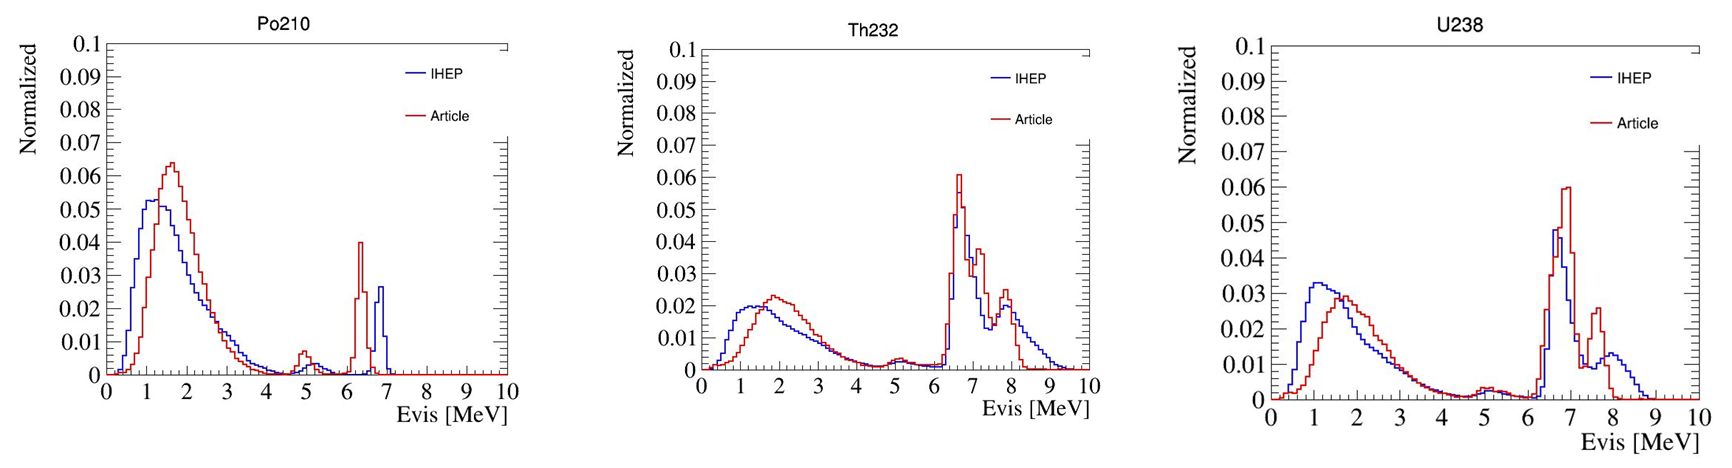
\includegraphics[width=16cm]{3_background/alphaNspec.png}
    \caption{Comparison of alphaN prompt spectrum from two generators.}
    \label{fig:alphaNspec}
\end{figure}

\subsubsection{Alpha rate}
The rates of $^{238}$U, $^{232}$Th are measured by BiPo correlated signal selection, details about the selection methods are described in Doc14623 and Doc14613. The rate of $^{210}$Po is measured by fitting the alpha peak in the total spectrum, details can be found in Doc14616.

The evolution of $^{214}$BiPo and $^{212}$BiPo are shown in Figure~\ref{fig:UTh}. The radon in LS in the begining is high, which lead to higher BiPo rate. The $^{214}$BiPo and $^{212}$BiPo have reached equilibrium states now, and the expected plateau are (7.5$\pm$0.9)$\times$10$^{-17}$ g/g for $^{238}$U and (8.2$\pm$0.7)$\times$10$^{-17}$ g/g for $^{232}$Th.

\begin{figure}[h]
    \centering
    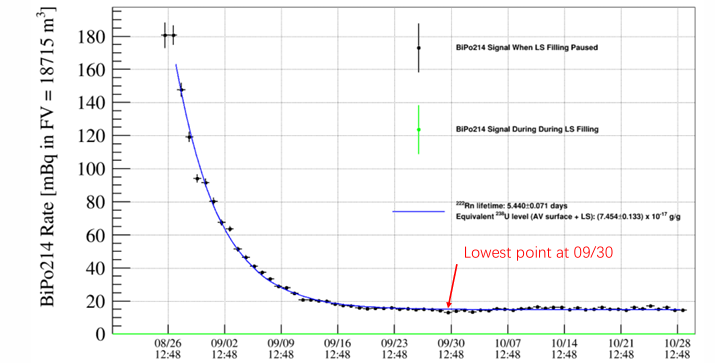
\includegraphics[width=8cm]{3_background/U238_update.png}
    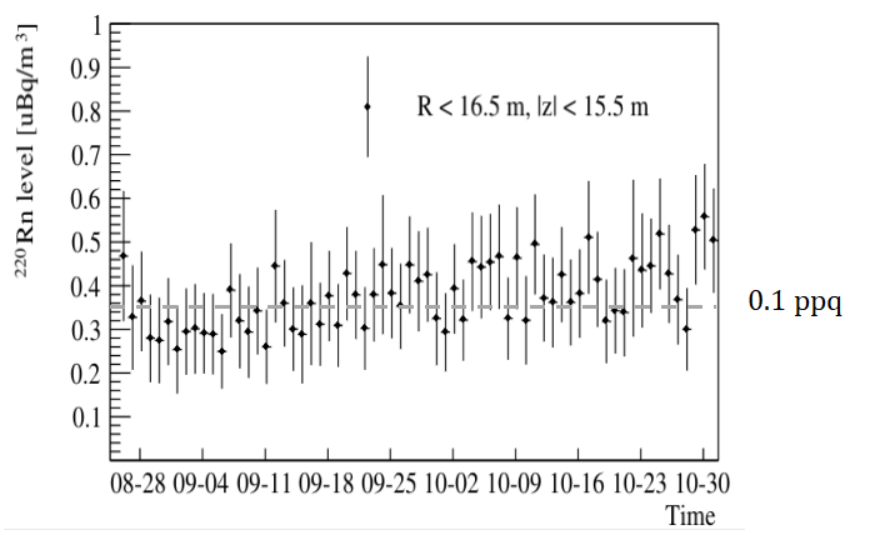
\includegraphics[width=9cm]{3_background/Th232_update.png}
    \caption{The evolution of $^{238}$U and $^{232}$Th within IBD FV cut (R<16.5m, |z|<15.5m).}
    \label{fig:UTh}
\end{figure}



The evolution of $^{210}$Po is shown in Figure~\ref{fig:Po210}. The half-life of $^{210}$Po is 138.376~days, thus the decay is slower and not reach equilibrium at present. The amount of $^{210}$Po was measured at the end of the LS filling at about 5$\times$10$^4$~cpd/kt, decreasing to an average (4.3$\pm$0.3)$\times$10$^4$~cpd/kt over the first two months of science runs.


\begin{figure}
    \centering
    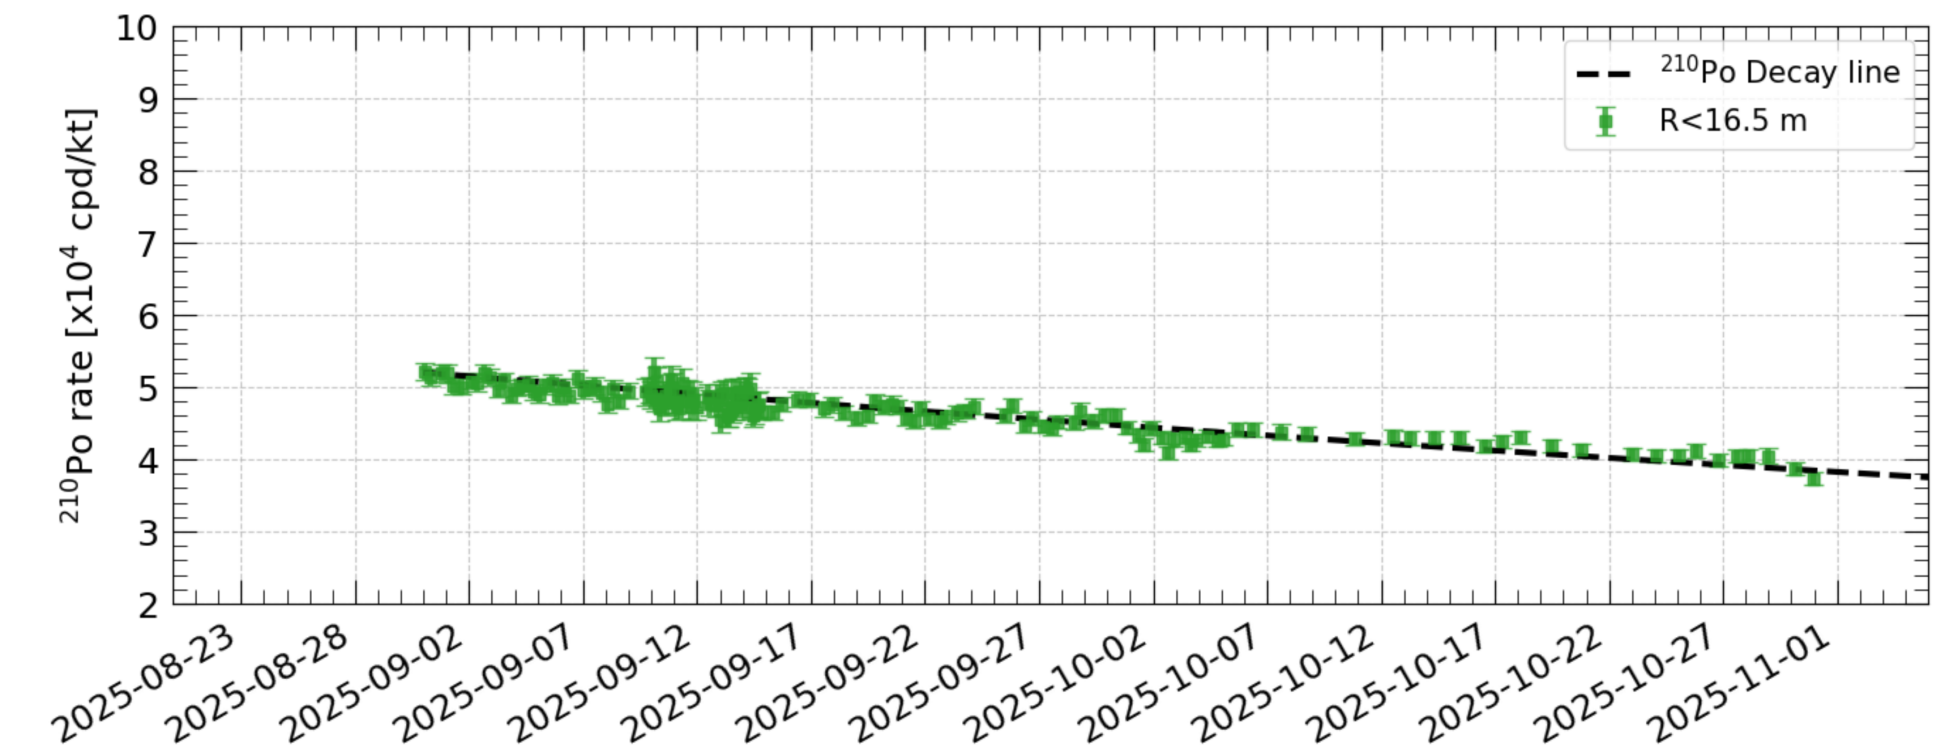
\includegraphics[width=0.75\linewidth]{3_background/Po210_update.png}
    \caption{The evolution of $^{210}$Po within IBD FV cut (R<16.5m).The black dashed line represents the $^{210}$Po decay curve, and its variation trend is quite consistent with that of the rate.  }
    \label{fig:Po210}
\end{figure}

\subsubsection{Final alphaN background rate}
With the calculated neutron yield from Table~\ref{tab:alphaNyield} and measure alpha rate, the final alphaN background rate is summarized in Table~\ref{tab:alphaN}.

% \begin{table}[!htbp]
%     \caption{Final alphaN background rate and uncertainty.}
%     \label{tab:alphaN}
%     \centering
%     \footnotesize% fontsize
%     \setlength{\tabcolsep}{4pt}% column separation
%     \renewcommand{\arraystretch}{1.2}%row space 
%     \begin{tabular}{c|cc|cc|cc}
%         \hline
%         \multirow{2}{*}{Alpha source} & \multicolumn{2}{c|}{Neutron yield [10$^{-7}$]} & \multicolumn{2}{c|}{Decay rate [cpd]} & \multicolumn{2}{c}{AlphaN rate [cpd]}  \\ \cline{2-7}
%         & value & uncertainty & value & uncertainty & value & uncertainty  \\ \hline
%         $^{238}$U & 6.36 & 25\% & 2.19 $\times 10^3$ & 10\% &1.5 $\times 10^{-3}$ & 27\% \\
%         $^{232}$Th & 8.58 & 25\% &68 & 16\% & 4.4 $\times 10^{-4}$& 30\% \\ 
%         $^{210}$Po & 0.613 & 25\% &7.8 $\times 10^5$ & 5\% & 4.4 $\times 10^{-2}$& 25\% \\
%         \hline 
%     \end{tabular}
% \end{table}

\begin{table}[!htbp]
    \caption{Final alphaN background rate and uncertainty.}
    \label{tab:alphaN}
    \centering
    \footnotesize% fontsize
    \setlength{\tabcolsep}{4pt}% column separation
    \renewcommand{\arraystretch}{1.2}%row space 
    \begin{tabular}{c|cc|cc|cc}
        \hline
        \multirow{2}{*}{Alpha source} & \multicolumn{2}{c|}{Neutron yield [10$^{-7}$]} & \multicolumn{2}{c|}{Decay rate [cpd]} & \multicolumn{2}{c}{AlphaN rate [cpd]}  \\ \cline{2-7}
        & value & uncertainty & value & uncertainty & value & uncertainty  \\ \hline
        $^{238}$U & 6.36 & 25\% & 2.2 $\times 10^3$ & 12\% &1.5 $\times 10^{-3}$ & 27\% \\
        $^{232}$Th & 8.58 & 25\% &64 & 9\% & 4.1 $\times 10^{-4}$& 27\% \\ 
        $^{210}$Po & 0.613 & 25\% &7.5 $\times 10^5$ & 7\% & 4.3 $\times 10^{-2}$& 25\% \\
        \hline 
    \end{tabular}
\end{table}

\subsection{World reactor neutrinos}
%By Rongping.

The main IBD signals of reactor antineutrinos are from the Yangjiang and Taishan NPPs, but there are also other more remote reactors all around the world.
In Table~\ref{tab:WR-1000}, we have listed the IBD rates of several reactors from world reactor contributions, with the distance less than 1000 km.
\begin{table}[!htbp]
    \caption{IBD rates of several reactors from world reactor contributions\textcolor{red}{(with an nominal efficiency of 82\%)}.}
    \label{tab:WR-1000}
    \centering
    \footnotesize% fontsize
    \setlength{\tabcolsep}{4pt}% column separation
    \renewcommand{\arraystretch}{1.2}%row space 
    \begin{tabular}{c|c|c|c|c}
        \hline
        Reactors & Core numbers & Distance (km) & Thermal Power (${\rm GW}_{\rm th}$) & Rate (cpd)\\ \hline
        FangChengGang & 4 & 411 & $2.905\times2+3.150\times2$ & 0.45\\
        ChangJiang & 2 & 478 & $1.930\times2$ & 0.13\\
        ZhangZhou & 1 & 543 & $3.150\times1$ & 0.08 \\
        FuQing & 6 & 796 & $2.905\times4+3.050\times2$ & 0.21 \\
        NingDe & 4 & 956 & $2.905\times4$ & 0.09\\
        \hline 
    \end{tabular}
\end{table}

From the Common Input for reactor neutrino analysis (and also in NMO and geo-neutrino sensitivity studies), we have considered the neutrino signal from the nearby reactors up to 300 km as the signal, including those from Yangjiang, Taishan and Daya Bay reactors, yet neutrinos from other remote nuclear power plants are usually defined as the world reactors, and will be the background for the oscillation analysis (Scenario A).

There is another scenario (Scenario B) that treats all the reactors up to 500 km as the signal, including additional contribution from FangChengGang and ChangJiang reactors, because weekly reactor running information will be available for all reactor cores within 500 km away from the JUNO site.

In scenario A (Scenario B), it will contribute 1.48 (0.90) IBD events per day \textcolor{red}{with an nominal efficiency of 82\% (same as the NMO paper and common inputs)}.

To calculate the world reactor neutrinos, We employ two main sources of information on the nuclear power plants and their running status, one is the International Atomic Energy Agency (IAEA), the other one is China Nuclear Energy Association (CNEA).
The former can provide the yearly and monthly running information for commercial and research reactors worldwide, and the latest effective duty factors until the end of 2024 are available. For CENA, quarterly information on reactors in mainland China can be obtained until the third quarter of 2025.%  June of 2025. Information of the third quarter will be online soon.

The time evolution of the world reactor neutrinos from IAEA are shown in Fig.~\ref{fig:WR-time-1}, where one can read that the event rate is steadily increasing and the ratio of those from Mainland China is also increased from 60\% to 80\%. Meanwhile, one can also calculate the world reactor neutrinos by replacing the information of reactors from Mainland China with CENA information, which is illustrated quarterly in Fig.~\ref{fig:WR-time-2}.
\begin{figure}%[h]
    \centering
    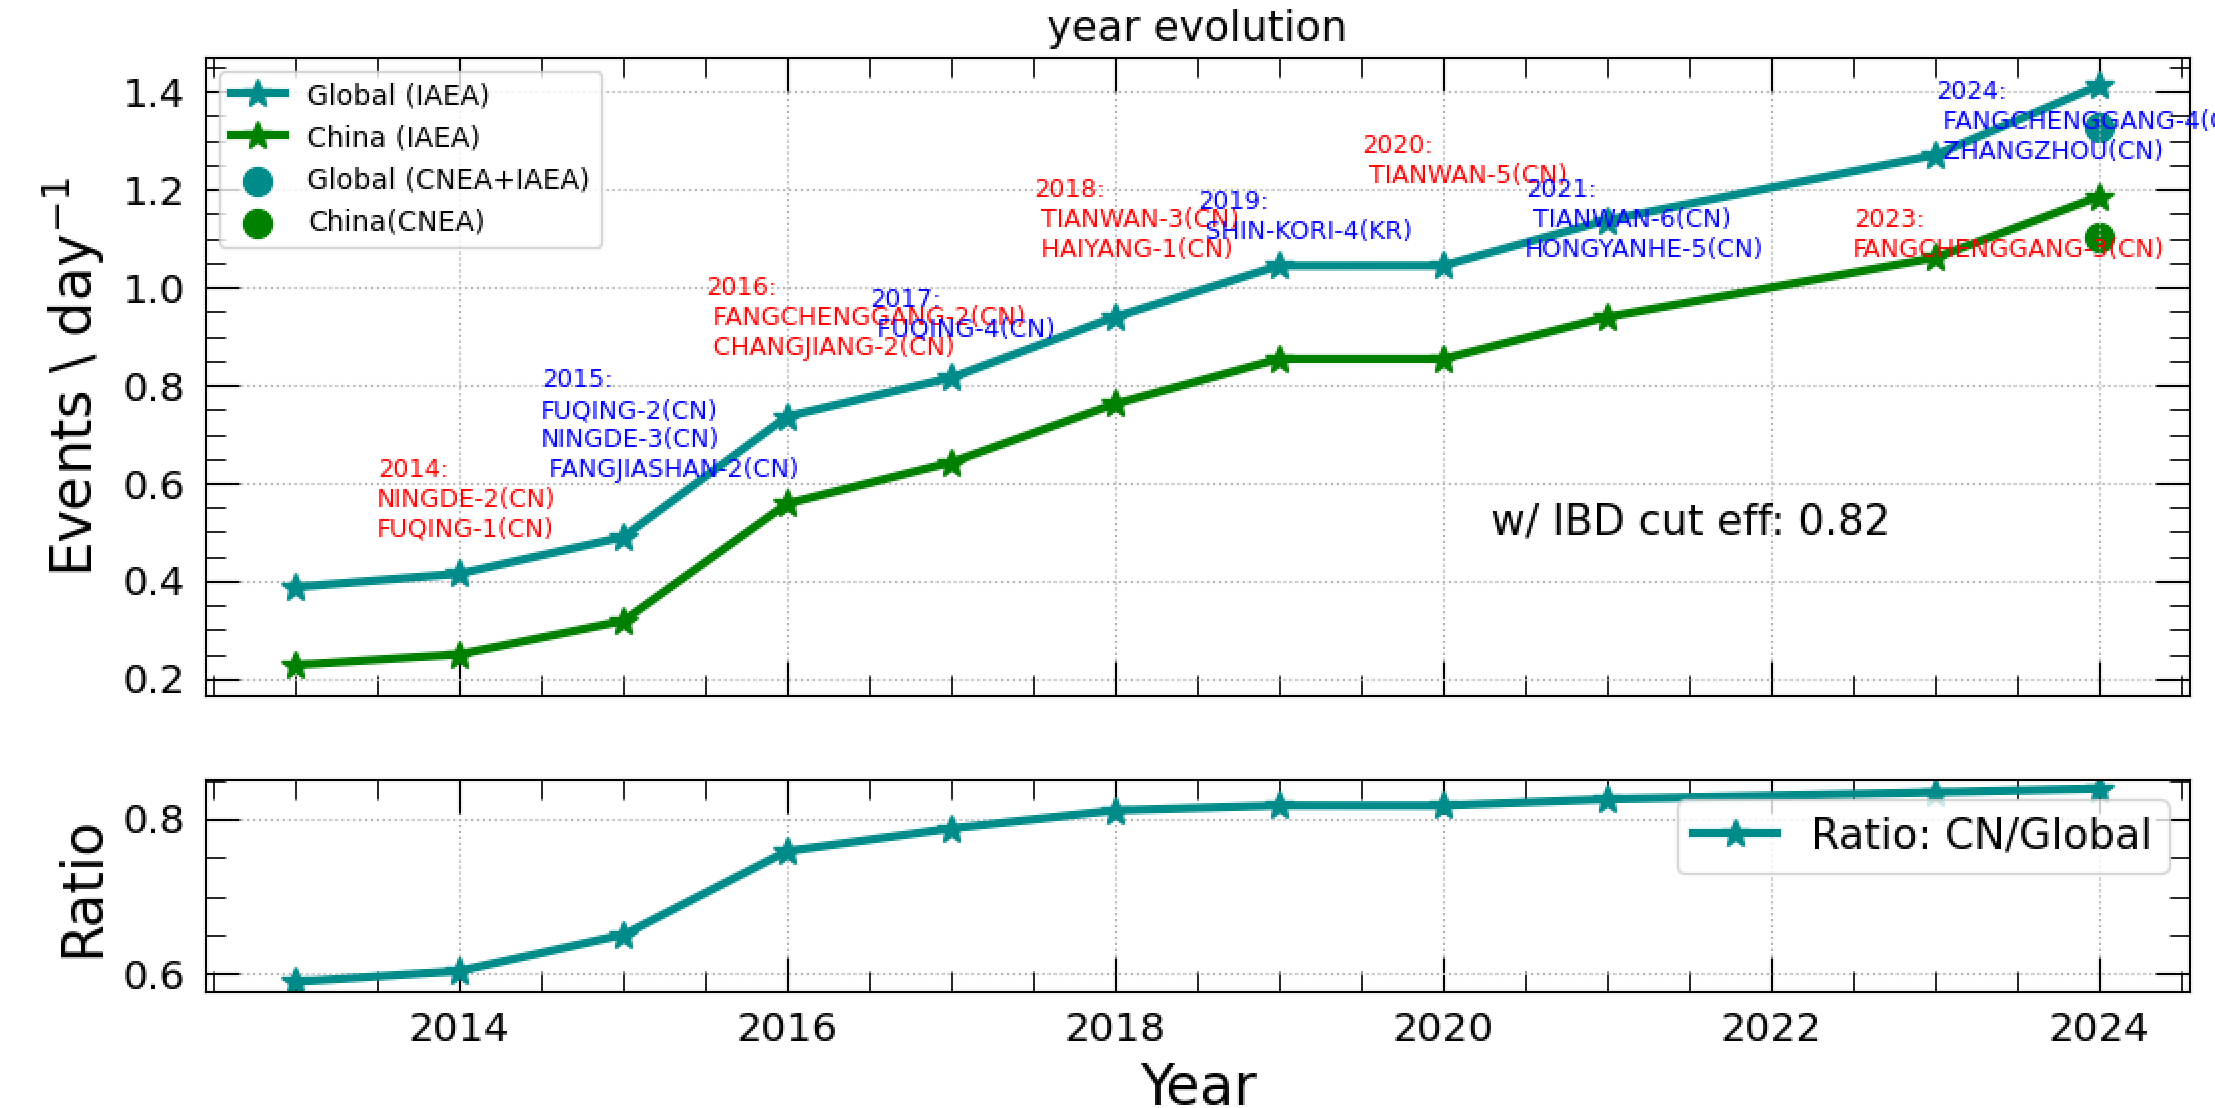
\includegraphics[width=0.75\linewidth]
    {3_background/Time_evolution-1_update.png}
    \caption{The yearly time evolution of IBD events from world reactor neutrinos \textcolor{red}{(with an nominal efficiency of 82\%)}.}
    \label{fig:WR-time-1}
\end{figure}


% \begin{figure}[h]
%     \centering
%     \includegraphics[width=0.75\linewidth]
%     {3_background/Time-evolution-2_update.png}
%     \caption{The quarterly time evolution of IBD events from world reactor neutrinos \textcolor{red}{(with an nominal efficiency of 82\%)}.}
%     \label{fig:WR-time-2_1}
% \end{figure}

\begin{figure}
    \centering
    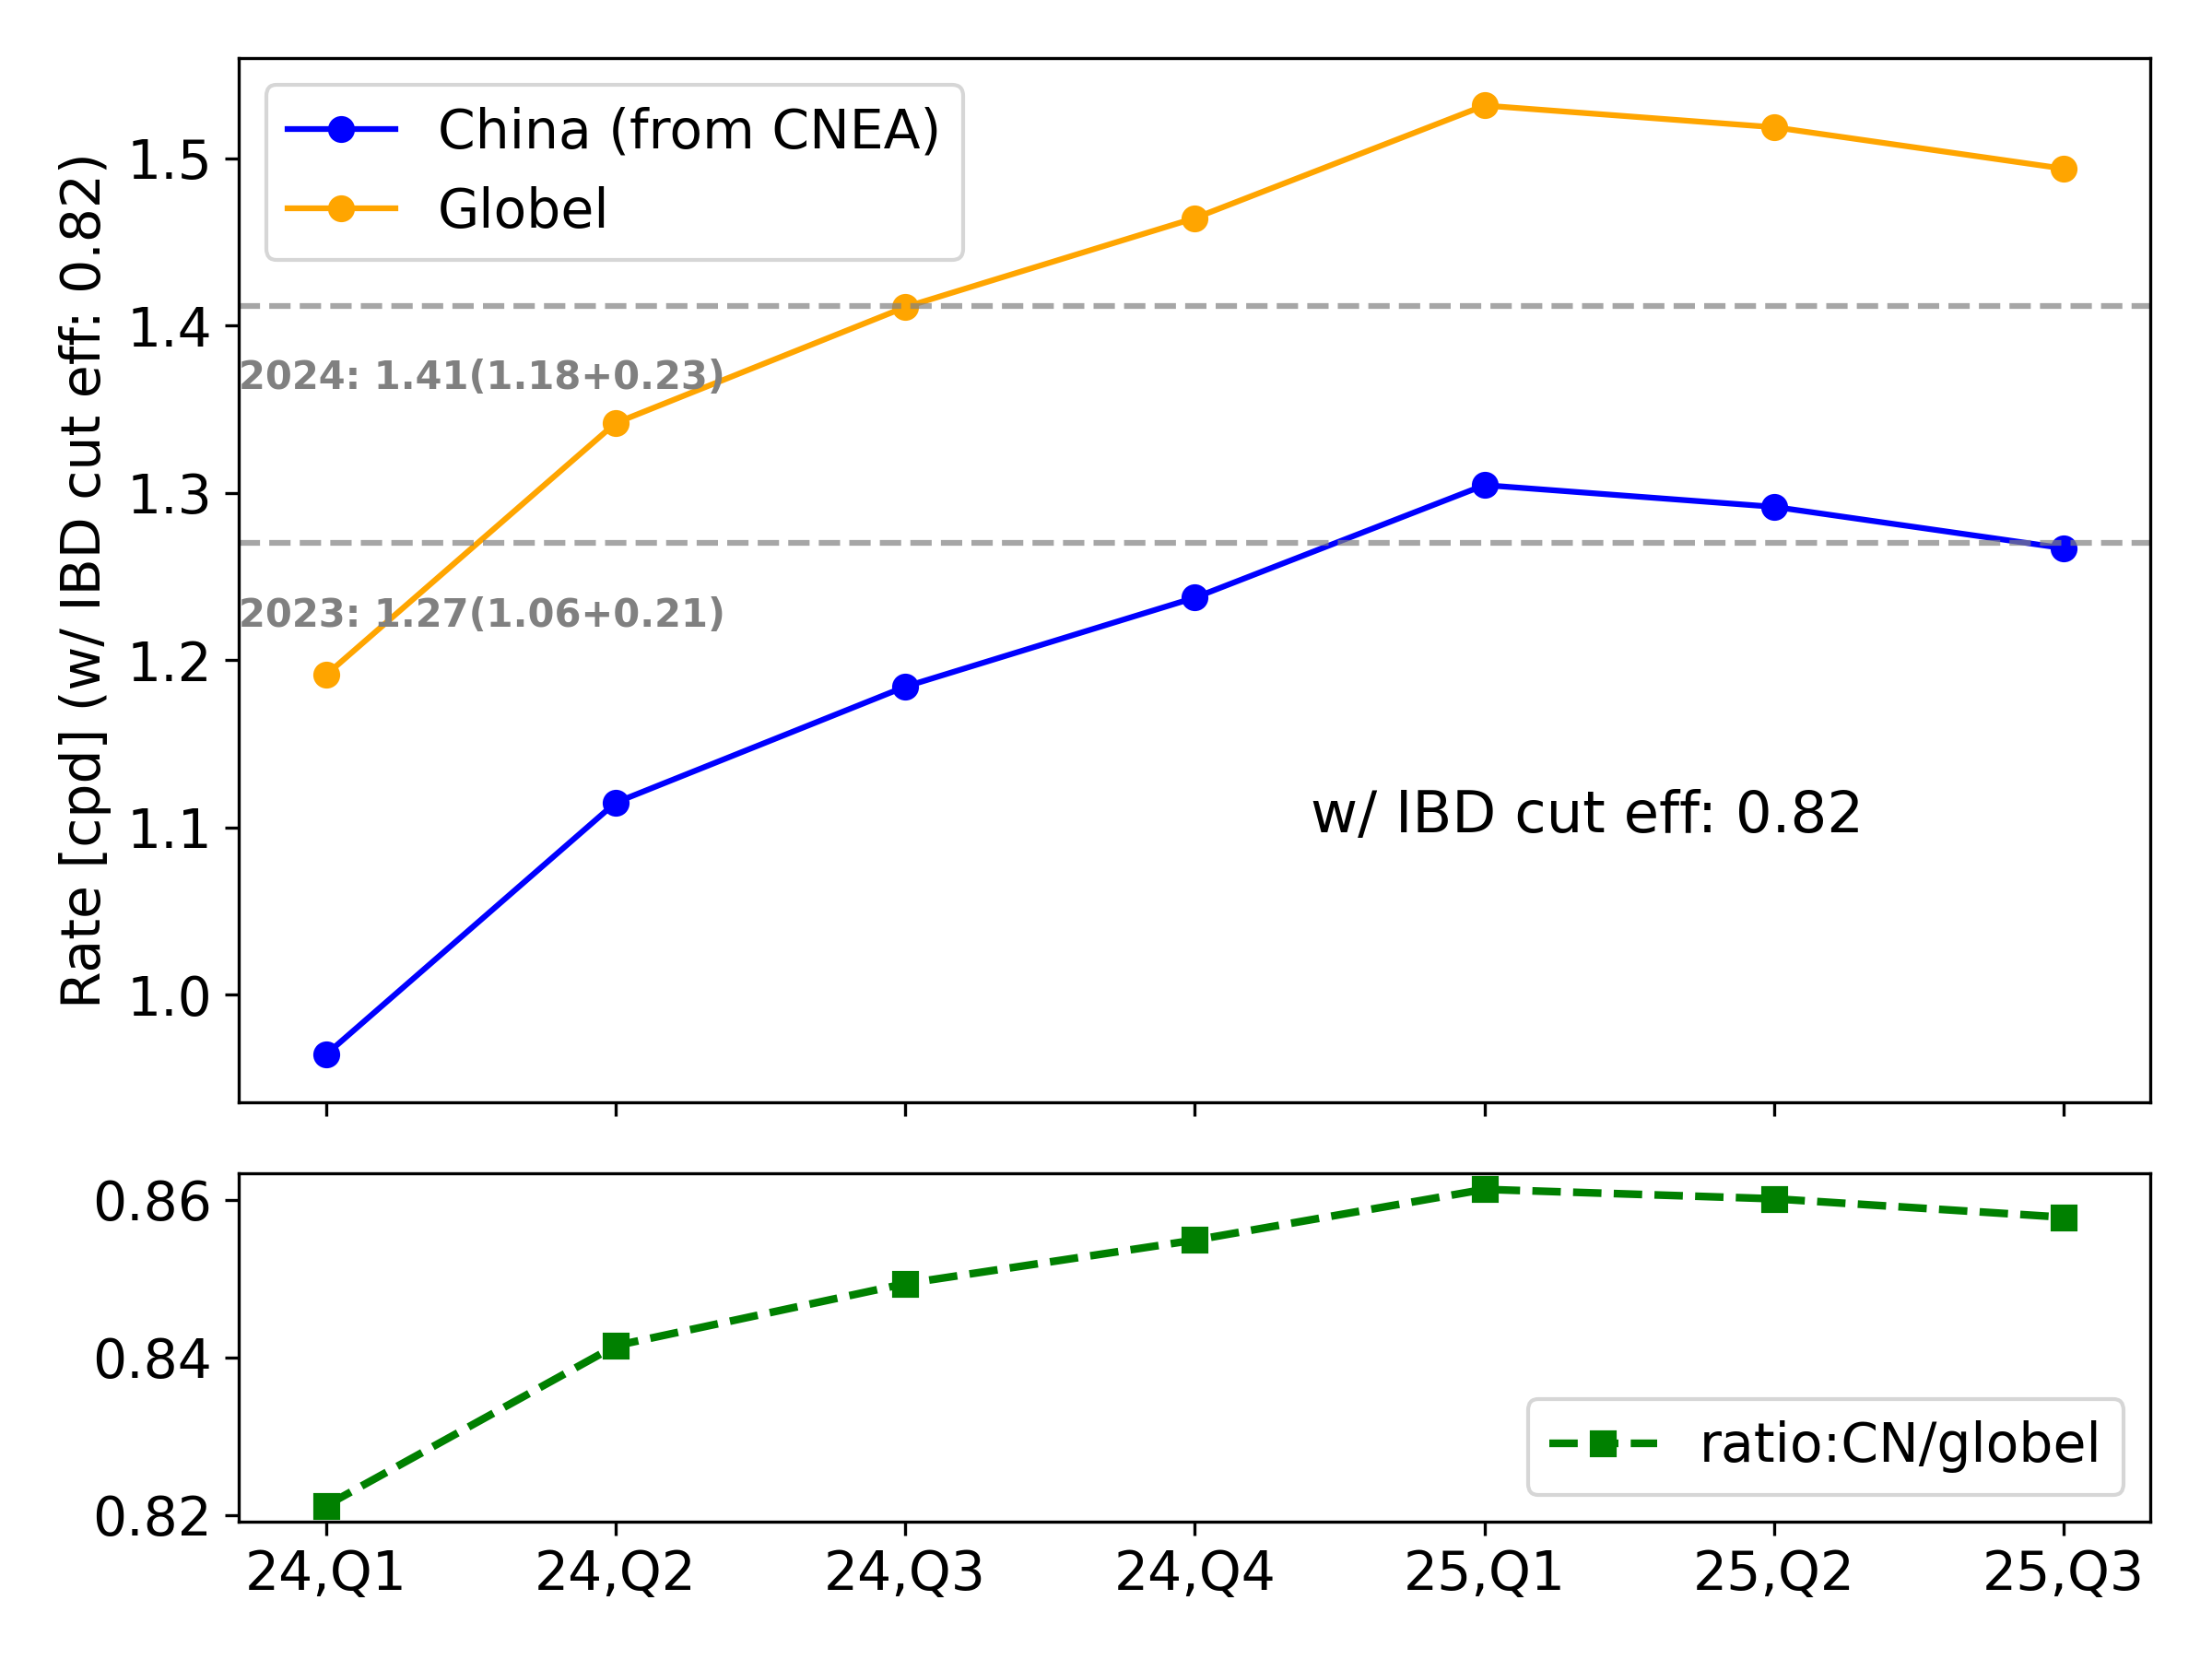
\includegraphics[width=0.75\linewidth]{3_background/time_evolution-3_update.png}
    \caption{The quarterly time evolution of IBD events from world reactor neutrinos \textcolor{red}{(with an nominal efficiency of 82\%)}.}
    \label{fig:WR-time-2}
\end{figure}




\begin{figure}[h]
    \centering
    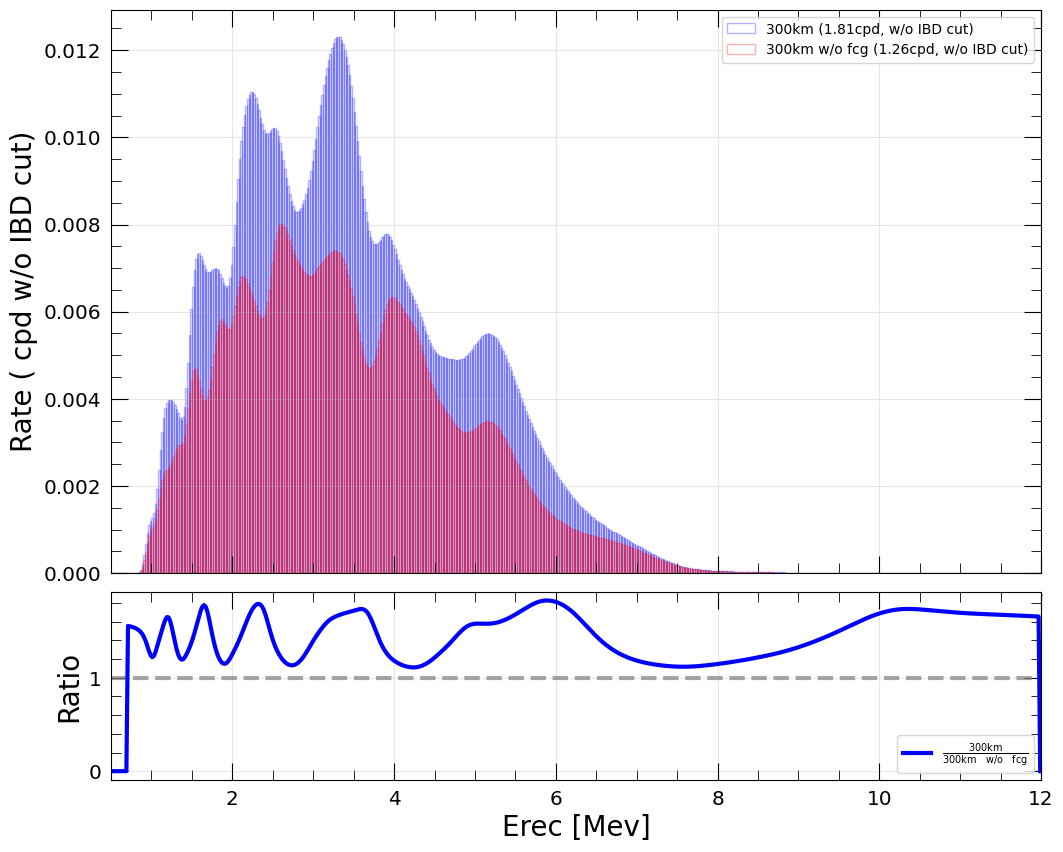
\includegraphics[width=0.7\linewidth]
    {3_background/time_evolution_update_251211}
    \caption{The spectrum shape of the IBD events from world reactor neutrinos. The detector response including energy resolution has been used.}
    \label{fig:WR-shape}
\end{figure}



From the time evolution study, we can conclude that contributions from reactors outside of mainland China are rather stable and the information in 2024 should be accurate enough for the current study. one the other hand, the reactor information for nearby reactors inside China should be as latest as possible. From Fig.~\ref{fig:WR-time-2}, we can observe that the first half year of 2025 is rather stable, and we are waiting for the third quarter release. 
Finally the reactors from Taiwan, China are absence from either of the above sources, thus we assume a distance of 1000 km and an effective thermal power of 10 ${\rm GW}_{\rm th}$.

We also calculate the neutrino events from research reactors from IAEA, and obtain the rate of $1.5\times10^{-3}$ cpd, which can be negligible.

By taking the duty factor information for the second quarter of 2025 in CNEA and all the others for the average one of 2024 in IAEA, we can calculate the event rate of world reactor neutrinos as 1.48 cpd \textcolor{red}{with an nominal efficiency of 82\%}. The spectrum shape of the world reactor neutrinos is shown in Fig.~\ref{fig:WR-shape}, and the detector response including energy resolution has been used. From the figure one can observe that the oscillation effect is still significant.

For the uncertainty evaluation, we mostly follow the method for the signal part, but the exception is the fission fraction is not known and one can only rely on the typical burnup period to make an educated guess. Since the fission fraction range of $^{235}{\rm U}$ could vary from 75\% to 50\%, we emply a half range of around 12\% to evaluate its induced uncertainty (see DocDB: 13065).
For Scenario A, by combining the uncertainty of thermal power (0.5\%), fission fraction (1.1\%), IBD yield (2\%) and detection (1.8\%) induced uncertainties, \textcolor{red}{we can have the total rate uncertainty of 3\%. Finally, considering the time delay of available reactor information, we would like to enlarge the rate uncertainty to 10\%}. The shape uncertainty is mainly from isotopic spectra from four isotopes. \textcolor{red}{It is evaluated as 5\%} from the theoretical model consideration (see DocDB: 5929), thus will keep unchanged for different binning scheme.
An alternative evaluation using the data driven method (from DYB data) will be provided soon.

Finally we want to comment that the oscillation effect is fixed when the world reactor neutrinos are considered as the background.
This may induce bias for the oscillation parameters when the true parameters are different from the current PDG central values. 
A study by comparing the world reactor neutrinos as either the signal (oscillation is properly considered for all reactors) or the background of Scenario A (the oscillated spectrum is fixed at the PDG central value) is employed and illustrated in Fig~\ref{fig:WR-bias}. The bias is around $0.05\sigma$ for 50 days of data, and will increase to $0.2\sigma$ for 6 years.
\begin{figure}[h]
    \centering
    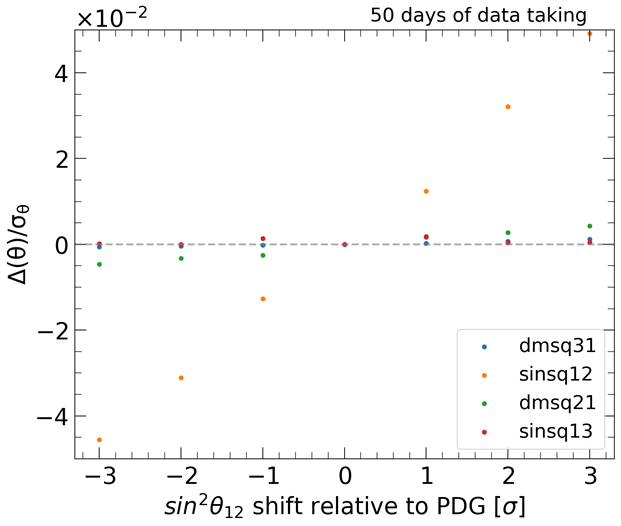
\includegraphics[width=0.7\linewidth]
    {3_background/WR-Bias-theta12.png}
    \caption{The induced bias of oscillation parameters by treating the world reactor neutrinos of further than 300 km (Scenario A) as fixed background, and assuming a shift of $\sin^2\theta_{12}$ relative the PDG value (bias induced by the shift of other parameters is smaller). The data taking time is 50 days.}
    \label{fig:WR-bias}
\end{figure}

\textcolor{red}{Given that the signal contribution from the Fangchenggang reactor accounts for a significant proportion of the overall signal from world reactors, and detailed operational information about this reactor is accessible, in our first paper, we incorporate Fangchenggang as a signal reactor (building upon the existing set of signal reactors), while classifying other reactors located more than 300 km away as world reactors and the uncertainty is same with before.}
%Our plan for this analysis of 50 days data is to employ Scenario B, because it can both largely reduce the bias and take into account the availability of reactor information.
%A quantitative test for this option will be provided soon.


\subsection{Geo-neutrinos}
%By Rongping.

%Geo-neutrinos are produced 
Geo-neutrinos are generated from the beta decay chains of the nuclear isotopes with long half-lives such as $\Um$, $\Th$, and $\K$ inside the Earth. At the JUNO detector, only the geo-neutrinos from $\Um$ and $\Th$ are observable above the threshold energy of the inverse beta decay (IBD) reaction ($\bar{\nu}_e + p \to e^+ + n$).

To make the prediction for the geo-neutrino singal, we make a new assessment of individual geo-neutrino fluxes by using the summation method from the decay chains of $\Um$ and $\Th$. The integration of the updated nuclear database, consideration of forbidden transitions, and inclusion of higher-order corrections yield significant spectral deviation compared to the currently commonly used Enomoto fluxes.
Compared to the Enomoto flux model, the IBD yield will have a decrease of $3.47\%$ for $\Um$ and $9\%$ for $\Th$.
Meanwhile, the spectral comparison is shown in Fig.~\ref{fig:geoUTh}. The spikes come from small changes of the Q values of beta branches, and the shape distortion is due to the forbidden decay features. The spectra used in the fitting will be convoluted with the IBD interaction with neutron recoils, the detector response and resolution.
\begin{figure}[h]
    \centering
    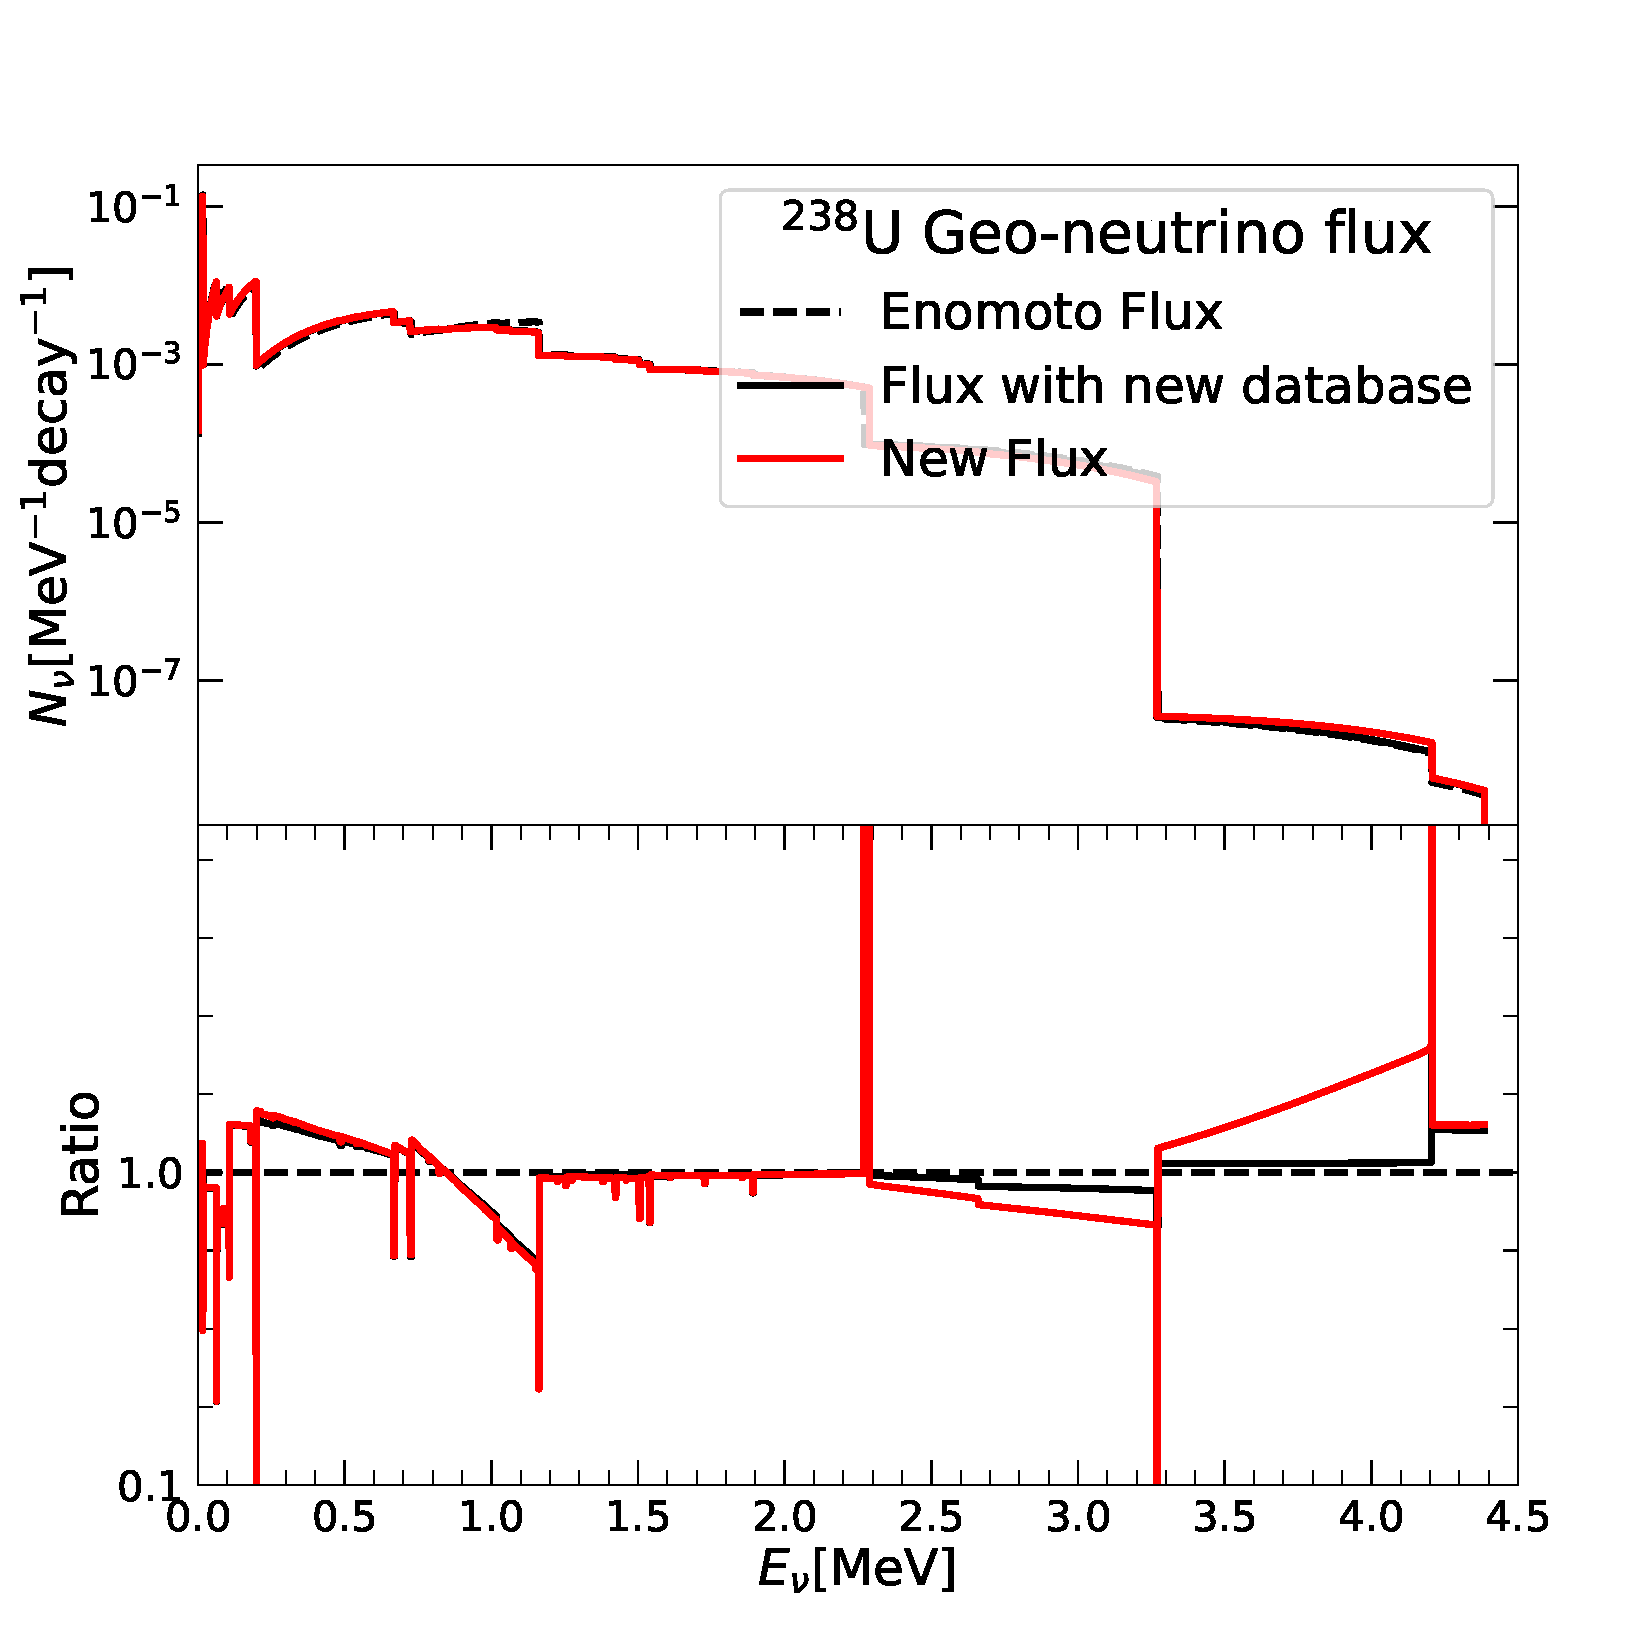
\includegraphics[width=8cm]{3_background/geoU238.pdf}
    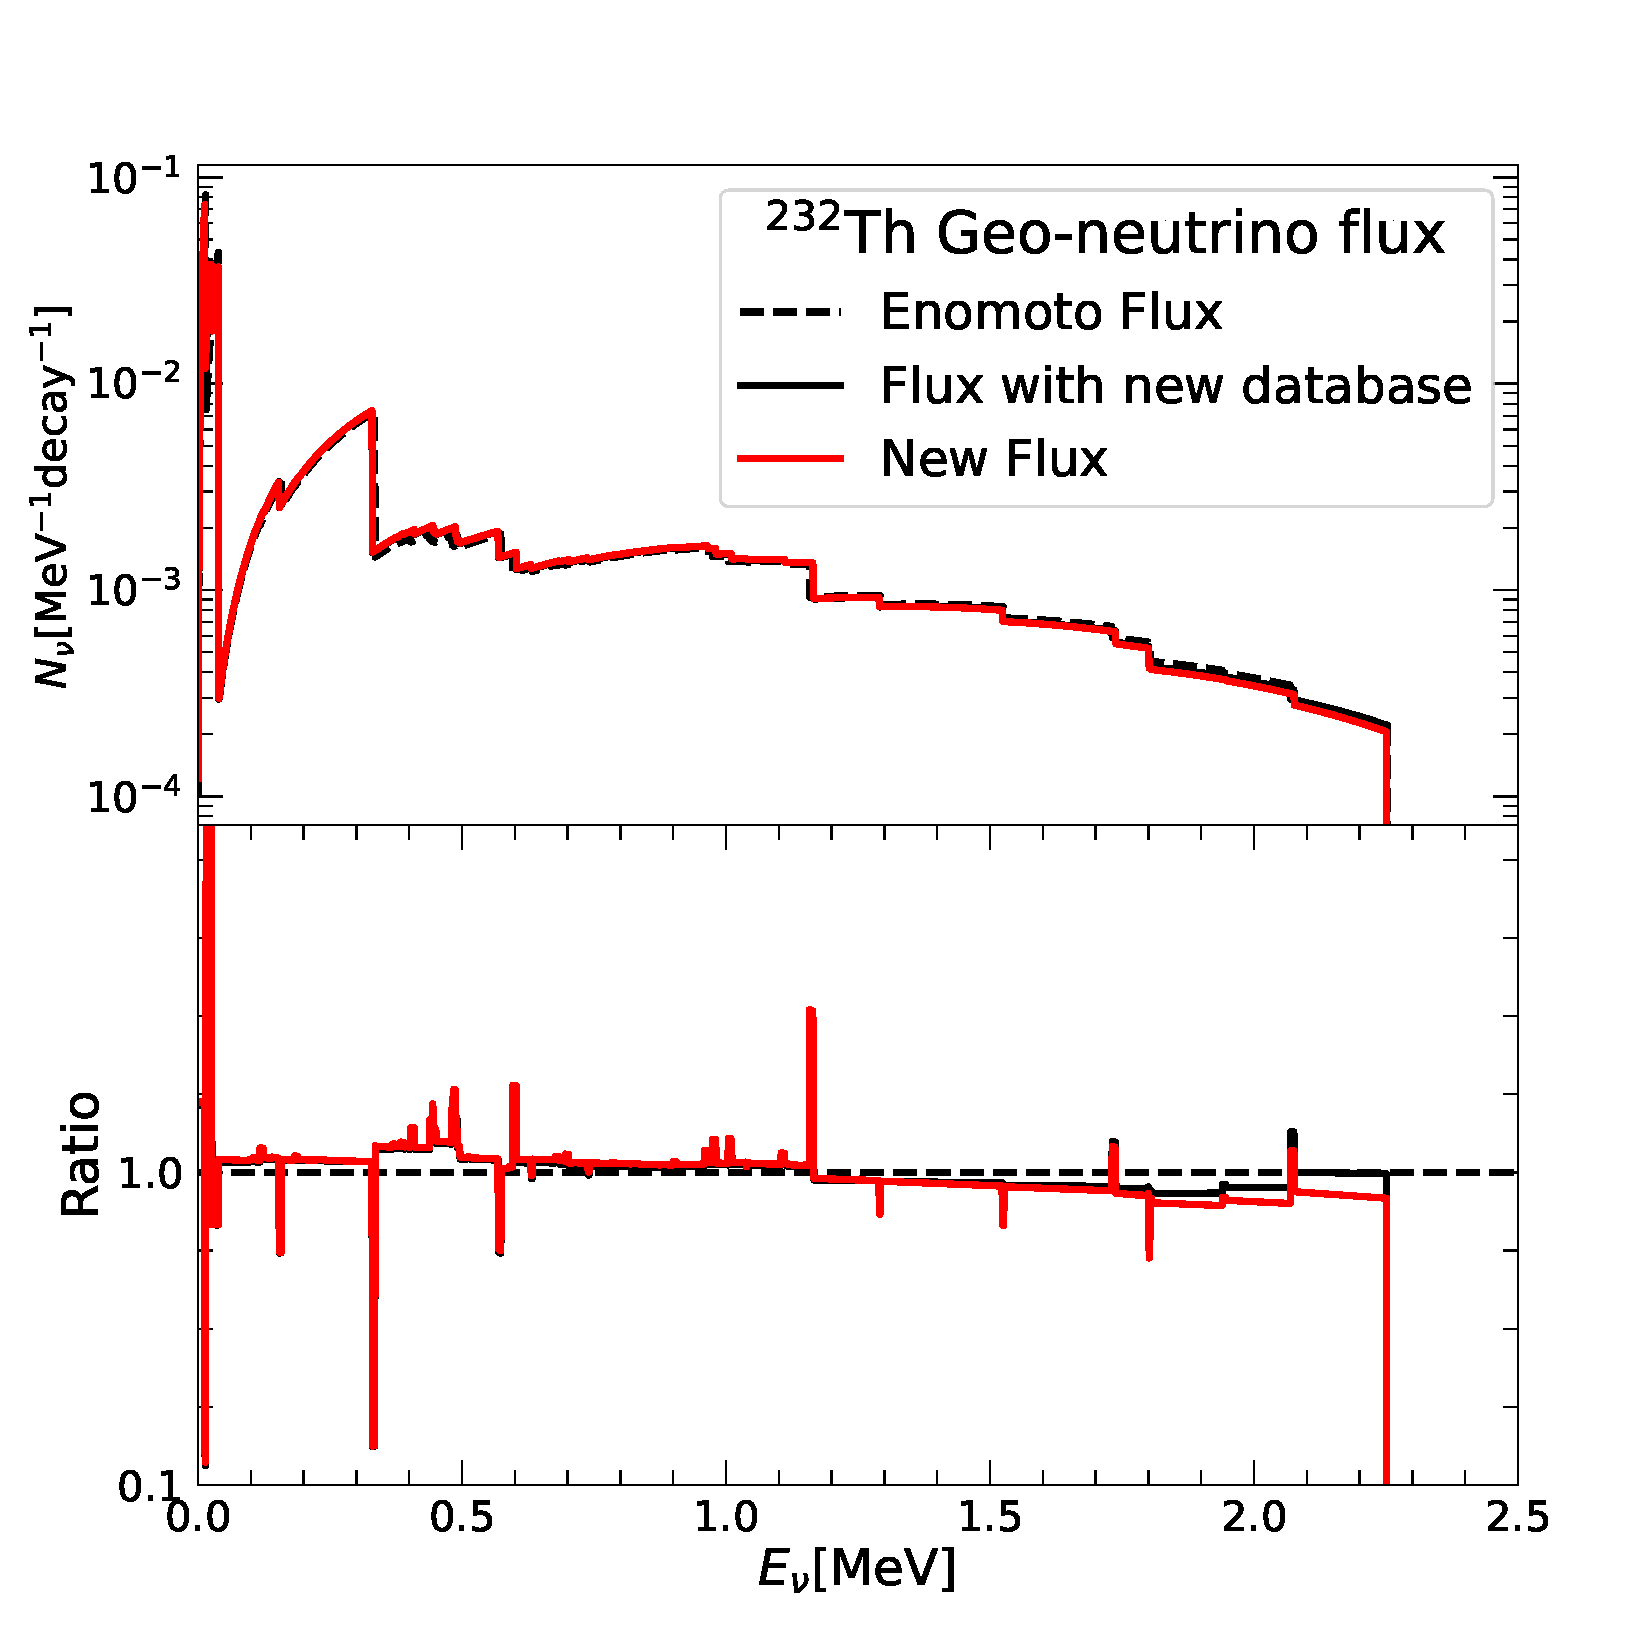
\includegraphics[width=8cm]{3_background/geoTh232.pdf}
    \caption{The geo-neutrino energy spectra from the decay chains of $\Um$ and $\Th$.}
    \label{fig:geoUTh}
\end{figure}

The rate of geo-neutrino signals depends on the inputs of geo-science information [see DocDB:13109, and tech-note and paper draft of geo-neutrino sensitivity paper DocDB: 14784]. For the crustal contribution, most of the variations are from either using the abundance of local rock samples near the JUNO site or the average values, in which the crust rates are ranged from $30.9^{+6.5}_{-5.2}$ TNU of the RRM model, to $40.4^{+5.6}_{-5.0}$ TNU of the JULOC model. For the mantle contribution, the variation are even larger, with three categories of poor-H, medium-H and rich-H models, having the rates of $\sim 2.8$ TNU, $\sim8.0$ TNU, and $\sim17.4$ TNU respectively. By directly combining the whole range of crustal and mantle contributions, the geo-neutrino rate can range from 27.5 TNU to 63.4 TNU. In order to cover the whole range and to be model independent, we choose the value  $44.3\pm18$ TNU [$1.75(1\pm40\%$) cpd](100\% efficiency). Note that totally free or 100\% uncertainty is an alternative choice.

% we choose the central value and half range as the rate uncertainty consideration, i.e., $45.5\pm18$ TNU [$1.4(1\pm40\%$) cpd]. Note that totally free or 100\% uncertainty is an alternative choice.

Typically we can choose a $\sim 5\%$ shape uncertainty for the database and beta decay uncertainty. The uncertainty from oscillation parameters is evaluated to be at the percentage level and can be included in the $5\%$ shape uncertainty. Note that the sensitivity of all parameters has negligible change when the shape uncertainty is increased to 20\% . 

\textcolor{red}{In our first paper, we also placed constraints on the U/Th ratio of the geoneutrino background, with an associated uncertainty of 10$\%$,and the center value of the ratio is 0.29.}

\subsection{Atmospheric neutrinos}
Atmospheric neutrino neutral current interaction with the carbon nuclei can knock out nucleons and introduce correlated IBD backgrounds. The event rate relative for reactor IBD analysis from such events were studied comprehensively in \cite{nc_epjc_2024}. Using state-of-the-art neutrino interaction models including GENIE (3.0.6) and NuWro (19.02), the impact on the event rate in the IBD energy region [0.7, 12] MeV due to nuclear models, final state interactions are studied. Using the avearge of five selected representing models, the nominal NC background rate is calculated to be 2.1$\pm$0.7 kton$^{-1}$yr$^{-1}$ (or 0.12$\pm$0.04 cpd in 20kton LS). The de-excitation of final state particles is implemented with a TALYS-based model. A 10\% rate difference is observed with de-excitation effect turned on and off. Therefore, a conservative 10\% rate error is assigned for de-excitation. Taking into another 10\% rate uncertainty from atmospheric neutrino flux, a total 50\% rate error is quoted.

The shape error is accounted by the shape-only distortion of each model w.r.t. the average model as 1$\sigma$ deviation \cite{nc_nominal}. Therefore, the NC background spectrum is treated in the following way:

\begin{equation}
    f(E) = A(f_0(E) + \sum_{i=1}^{5}a_if_i(E) )
\end{equation}

where $f_0(E)$ is the nominal model, $f_i(E)$ is the shape-only difference between the $i$-th model and the nominal model. $A$ is the rate nuisance parameter contrained to follow Gaus(1, 0.5) and $a_i$ follows Gaus(0, 1).

\subsection{Summary}
\begin{table}[!htbp]
    \caption{Summary of signal and backgrounds. The detection efficiencies are included. }
    \centering
    \footnotesize% fontsize
    \setlength{\tabcolsep}{4pt}% column separation
    \renewcommand{\arraystretch}{1.2}%row space
    %\resizebox{\linewidth}{!}{
    \begin{tabular}{lcc}
        \hline
          & Selection A1 & Shape uncertainty \\ 
        \hline
        $\overline{\nu}_{e}$ candidates & 2379 & - \\
        DAQ live time (days) & 59.08 & - \\
        Geoneutrinos (day$^{-1}$) & 1.23$\pm$0.49 & 5\% bin-to-bin + Th/U=0.29$\pm$0.03\\
        World reactors (day$^{-1}$) & 0.88$\pm$0.09 & 5\% bin-to-bin \\
        Accidentals (day$^{-1}$) & 0.049$\pm$0.003 & 20\% \\
        BiPo214 (day$^{-1}$) & 0.18$\pm$0.10  & 5\% \\
        Fast neutron (day$^{-1}$) & 0.02$\pm$0.02 & 60\% \\
        Double neutron (day$^{-1}$) & 0.05$\pm$0.05 & 50\% \\
        \Li~(day$^{-1}$) & 4.28$\pm$1.44 & 20\% \\
        %B12-B12 & <0.02 & xx \\
        Atmospheric neutrinos (day$^{-1}$) & 0.08$\pm$0.04 & Option2 in DocDB-14940 \\
        $^{13}$C ($\alpha, n$) $^{16}$O (day$^{-1}$) & 0.04$\pm$0.02  & 50\% bin-to-bin \\
        %$\overline{\nu}_{e}$ rate  (day$^{-1}$) & xx$\pm$xx & -\\
        \hline
    \end{tabular}
    %}
    \label{tab:selResults}
\end{table}


